\section{Background estimation technique}
\label{sec:alpha}

The goal of the analysis is to look for localized excesses in the \mtVZ spectrum. The \emph{$\alpha$-method} is used in searches for heavy resonances since Run 1~\cite{Khachatryan:2015cwa}, and it has been introduced to be less dependent on the MC simulation for the background \mtVZ estimation, due to the many sources of systematic uncertainties that are hard to understand and control. The two exclusive regions, \emph{signal region} (SR) and \emph{sidebands region} (SB), define a signal enriched or signal depleted phase space, respectively. First, the background normalization is extracted from data in the SB. Then, the $\alpha$-method extracts a predicted shape from the data in the SB to the SR using a transfer function (the $\alpha$ function) derived from simulation. The method relies on the assumption that the correlation between \mtVZ and the groomed jet mass is reasonably well reproduced by the MC. The $\alpha$ ratio is deemed to be more trustworthy since many systematic uncertainties would approximately cancel in the ratio.

\noindent Let's assume that, in the simplest case, only one dominant background is present. The $\alpha$ function is defined as the ratio of the two functions describing the simulated \mtVZ shape in the SR and SB:
%In the simplest case, only one dominant background is present. 

\begin{equation}
\alpha(\mtVZ) = \frac{f_{\text{SR}}^{\text{MC,bkg}}(\mtVZ)}{f_{\text{SB}}^{\text{MC,bkg}}(\mtVZ)}
\end{equation}

\noindent and the background distribution in the SR is thus estimated as the product of  $\alpha(\mtVZ)$ with the shape in the data SB:

\begin{equation}
f_{\text{bkg}}(\mtVZ) = f_{\text{SB}}(\mtVZ) \times \alpha(\mtVZ)
\end{equation}

\noindent In the above description, no definition of the SB and SR is included. Ideally, the best choice would be a variable such that the distribution of \mtVZ in the signal region and sidebands are similar. In this analysis, the soft drop PUPPI corrected jet mass $m_j$ (sec.~\ref{ssec:jetmass}) is chosen as the control variable, and the cut values are those reported in tab.~\ref{tab:SR-SB}. All the selections used in the $\alpha$ method background prediction are the same reported in sec.~\ref{ssec:final_dib_cand}.
%In order to respect the blinding policy of the diboson VV searches, the Higgs mass window is not used neither for the background estimation (it can be potentially contamined by a signal) nor as signal region.

\noindent In a real case scenario, the background is not purely composed of one single process neither in the SR nor in the SB. As already pointed out in sec.~\ref{ssec:backgrounds} and confirmed in sec.~\ref{sec:datamc_comp}, the background composition is dominated by two processes, \Z + jets ($\sim 50\%$ in the whole SR) and \W + jets ($\sim 35\%$ in the whole SR), grouped together as \V+jets, whose modeling in simulation is considered not to be trustworthy. Other subdominant backgrounds, \ttbar and single-t production, groupde as Top, and diboson (\VV), generally have smaller contributions (of the order of 5\% for \VV, and 9\% for Top, in the whole SR), and are considered quite well understood and modeled by MC generators. The justification of fixing \W + jets and \Z + jets is provided in sec.~\ref{ssec:alpha_validation}

\noindent The shape and normalization of the \VV and Top production is taken from the simulation. The sub-dominant backgrounds are then subtracted from the \V+jets contribution when fitting this template to data. The shape and normalization of the main background is evaluated with the $\alpha$ approach.

%One single $\alpha$ function is defined for each channel and category, that is obtained with the simulated background composition, and multiplied by the data distribution in the SB. This implies that the shape change between SB and SR does not heavily depend on the background process, and even if it does, the $\alpha$ function is already built with the expected ratio between various processes. With respect to the subtraction of the sub-dominant background, this choice has the advantage to take into account the shape variation also for the sub-dominant backgrounds, which can be non-negligible in some channels. Anyway, the normalization for the sub-dominant backgrounds is estimated separately due to the different jet mass distribution.

\noindent A different background prediction is derived for each category separately, thus dividing low- and high-purity categories, and it is calculated in a transverse mass range $950 <$ \mtVZ $<4750$ GeV.

\subsection{Background normalization}\label{ssec:alphaNorm}

The first step in the background prediction consists in a proper estimation of the background normalization. The three main backgrounds (\V+jets, Top, and \VV) are considered separately due to the different shape in the jet mass distribution. The three contributions are described with functional forms determined by fits on the simulated backgrounds. The so-built templates are summed together, maintaining the relative weights between the three, and finally fitted to the data in the jet mass sidebands. During the fit to data SB, the parameters of the \V + jets background are left free to float and adapt to the data distribution. The integral of the final sum of the fitted functions over the SR jet mass range represents the background normalization in the SR.
%The number of expected events in the SR is extracted through the following equation:

%\begin{equation}
%N_{\text{SR}}^{\text{data}} = \left[ N_{\text{SB}}^{\text{data}} - N_{\text{SB}}^{\text{Top}} - N_{\text{SB}}^{\text{VV}} \right]  + N_{\text{SR}}^{\text{Top}} + N_{\text{SR}}^{\text{VV}}
%\label{eq:alpha_norm}
%\end{equation}
%where in this case $N$ are the number of events, and not functions.

\noindent The empirical functional forms for each background are chosen to reflect the physics properties of the samples. In the low-purity category, the \V+ jets background is a falling background with no peaks, modelled as a power law, while in the high-purity category the \V+jets background component is characterized by a broad distribution roughly centered at $m_\V$, modelled as a gaussian, with an exponential tail at high mass values. The exponential falling \VV $m_j$ spectrum shows a peak, corresponding to the vector boson hadronic decay reconstruction, that is modelled as a gaussian. The hadronic decays of \W and \Z bosons cannot be distinguished, hence they are fitted together. For the jet mass spectrum of the Top backgrounds, the peaks corresponding to the $W$ and top quark mass can be modelled as gaussian functions, superimposed to a falling exponential background.

\noindent The functional forms chosen to build the jet mass templates are:

\begin{itemize}
  %%\item[{\bf Exp}:] an exponential function: $$F_{\rm Exp}(x)=e^{ax}$$
  %%\item[{\bf Pol}:] a third order polynomial: $$F_{\rm Pol}(x)=a_0 \cdot x + a_2 \cdot x^2 + a_3 \cdot x^3 $$
  %\item {\tt ErfExp}: an exponential multiplied by an ``error function'' {\tt Erf}: $$F_{\rm ErfExp}(x)=e^{ax} \cdot \frac{1 + {\rm Erf}((x-b)/w)}{2}$$ %an exponential times an ``error function'', that consists of 
  %\item {\tt ErfExpTail}: an {\tt ErfExp} modified to account for an additional term in the exponential, that results in a tail ad high masses: $$F_{\rm ErfExpTail}(x)=e^{-x/(a+b*x)} \cdot \frac{1 + {\rm Erf}((x-o)/w)}{2}$$
  \item {\tt ErfPow2}: an error function ({\tt Erf}) multiplied by a power law: $$F_{\rm ErfPow2}(x)={ \left( \frac{x}{\sqrt{s}} \right)}^{- c_0 + c_1 \log(x/\sqrt{s})} \cdot \frac{1 + {\rm Erf}((x-o)/w)}{2}$$
  %
  %\item[{\bf Gaus}:] one gaussian: $$F_{\rm Gaus}(x) = \cdot e^{2(x-a)^2/b}$$
  %\item[{\bf Gaus2}:] two gaussians: $$F_{\rm Gaus2}(x) = f_0 \cdot e^{2(x-a)^2/b} + (1-f_0) \cdot e^{2(x-c)^2/d}$$
  %\item {\tt Gaus3}: three gaussians: $$F_{\rm Gaus3}(x) = f_0 \cdot e^{2(x-a)^2/b} +f_1 \cdot e^{2(x-c)^2/d} + (1-f_0-f_1) \cdot e^{2(x-e)^2/g}$$
  %
  \item {\tt ExpGaus}: an exponential plus one gaussian: $$F_{\rm ExpGaus}(x) = f_0 \cdot e^{ax} + (1-f_0) \cdot e^{2(x-b)^2/c}$$
  %\item[{\bf ExpGaus2}:] an exponential plus two gaussians: $$F_{\rm ExpGaus2}(x) = f_0 \cdot e^{ax} + f_1 \cdot e^{2(x-b)^2/c} + (1-f_0-f_1) \cdot e^{2(x-d)^2/e}$$
  \item {\tt ErfExpGaus}: an error function plus one gaussian: $$F_{\rm ErfExpGaus}(x) = f_0 \cdot F_{\rm ErfExp}(x,a,b,c) + (1-f_0) \cdot e^{2(x-d)^2/e}$$
  \item {\tt ErfExpGaus2}: an error function plus two gaussians: $$F_{\rm ExpGaus2}(x) = f_0 \cdot F_{\rm ErfExp}(x,a,b,c) + f_1 \cdot e^{2(x-d)^2/e} + (1-f_0-f_1) \cdot e^{2(x-f)^2/g}$$
\end{itemize}

\noindent The choice of the functions is channel-dependent, and it depends on the background shape and the available statistics, and is summarized in tab.~\ref{tab:MassFunctions}. In order to make the background evaluation less dependent as possible from the choice of the function describing the jet mass of the main background, an alternative function has been used to fit the \V + jets background. The absolute difference bewteen the number of expected events calculated with the main \V + jets function and the alternative is taken as systematic uncertainty.

\begin{table}[!htb]
  \begin{center}
    \begin{tabular}{c|ccccc}
      category & \V+jets & alt. \V+jets & Top & VV \\
      \hline
      \hline
      low-purity  & ErfPow2 & ExpGaus & ErfExpGaus2 & ExpGaus \\
      \hline
      high-purity & ExpGaus & ErfExpGaus & ErfExpGaus2 & ExpGaus \\
    \end{tabular}
  \end{center}
  \caption{Chosen functions to fit the jet mass distribution for each channel.}\label{tab:MassFunctions}
\end{table}

\begin{table}[!htb]
  \begin{center}
    \begin{tabular}{cc|c|ccc|c}
      Region & Category   & Expected & Statistical       & Systematic     & Alternative function& Observed \\
       &  & events & uncertainty       & uncertainty     & uncertainty & events\\
      \hline
      \hline
      SB     & low-purity & $2356.6$ & $\pm 52.5$ & $\pm 16.0$ & $\pm 1.1$    & $2314$ \\
      SR     & low-purity & $1093.2$  & $\pm 48.1$ & $\pm 16.4$ & $\pm 49.1$   & $1153$ \\
      \hline
      SB & high-purity    & $779.8$  & $\pm 29.1$ & $\pm 13.1$ & $\pm 0.3$  & $774$ \\
      SR & high-purity    & $254.4$  & $\pm 15.3$ & $\pm 17.9$ & $\pm 7.8$  & $271$ \\
    \end{tabular}
  \end{center}
  \caption{Expected background yield in the SB ($30 < m_j < 65\GeV$, $m_j > 135\GeV$ )and in the SR ($65 < m_j < 105\GeV$) and relative uncertainties.}\label{tab:BkgNorm}
\end{table}

\noindent The following plots (fig.~\ref{fig:XVZnnlp_JetMass}-\ref{fig:XVZnnhp_JetMass}) show the fits to the jet mass distributions in Monte Carlo samples, in the different channels; the alternative functions for the main background are displayed with dotted lines. The background estimation, after the fit to data SB, is showed in fig.~\ref{fig:XVZnn_JetMass}. The bottom panels of each plot display the fit pulls (per-bin), namely, the number of events observed in data (or in Monte Carlo simulations) minus the number of events predicted by the fit, divided by the uncertainty in the data (or simulations). Table~\ref{tab:BkgNorm} summarizes the expected background yield in the signal region, that is in agreement with observation in both the purity categories. The quoted uncertainties are calculated as follows:
\begin{itemize}
\item the statistic uncertainty is the uncertainty of the fit to the \V + jet background;
\item the systematic uncertainty is the propagation of the uncertainties of the fits to the \VV and Top backgrounds;
\item the alternative function uncertainty describes the discrepancy in the background yield in SR depending on the choice of the function to describe the \V + jets background.
\end{itemize}

%[FIXME: numbers in table to be updated]



%\clearpage


%%% 2 electrons %%%

\begin{figure}[!htb]
  \centering
    \includegraphics[width=.33\textwidth]{v9/plotsAlpha/XVZnnlp/VjetMass.pdf}
    \includegraphics[width=.33\textwidth]{v9/plotsAlpha/XVZnnlp/VVMass.pdf}
    \includegraphics[width=.33\textwidth]{v9/plotsAlpha/XVZnnlp/TopMass.pdf}
  \caption{Fit to the simulated $m_j$ in the low-purity category for the three backgrounds: \V+jets (left), \VV (center), Top (right). For the main background prediction, the alternative function is displayed with a dotted red line, superimposed to the main choice (continuous light blue curve).}
  \label{fig:XVZnnlp_JetMass}
\end{figure}


\begin{figure}[!htb]
  \centering
    \includegraphics[width=.33\textwidth]{v9/plotsAlpha/XVZnnhp/VjetMass.pdf}
    \includegraphics[width=.33\textwidth]{v9/plotsAlpha/XVZnnhp/VVMass.pdf}
    \includegraphics[width=.33\textwidth]{v9/plotsAlpha/XVZnnhp/TopMass.pdf}
  \caption{Fit to the simulated $m_j$ in the high-purity category for the three backgrounds: \V+jets (left), \VV (center), Top (right). For the main background prediction, the alternative function is displayed with a dotted red line, superimposed to the main choice (continuous light blue curve).}
  \label{fig:XVZnnhp_JetMass}
\end{figure}


\begin{figure}[!htb]
  \centering
    \includegraphics[width=.495\textwidth]{v9/plotsAlpha/XVZnnlp/XVZnnlp_JetMass_U.pdf}
    \includegraphics[width=.495\textwidth]{v9/plotsAlpha/XVZnnhp/XVZnnhp_JetMass_U.pdf}
  \caption{Background yield prediction in the signal region, after the fit to data sidebands, in the low- (left) and high-purity category (right). Data and predictions are in agreement.}
  \label{fig:XVZnn_JetMass}
\end{figure}




%\clearpage




\subsection{Background shape}\label{ssec:alphaShape}

The second part of the background prediction consists in estimating the background shape of the transverse mass of the diboson candidate, \mtVZ. Each transverse mass spectrum is parametrized separately for the \V + jets ($f_{\text{SR}}^{\text{MC, \V + jets}}(\mtVZ)$, $f_{\text{SB}}^{\text{MC, \V + jets}}(\mtVZ)$), Top production ($f_{\text{SR}}^{\text{MC, Top}}(\mtVZ)$, $f_{\text{SB}}^{\text{MC, Top}}(\mtVZ)$), and dibosons ($f_{\text{SR}}^{\text{MC, VV}}(\mtVZ)$, $f_{\text{SB}}^{\text{MC, VV}}(\mtVZ)$). These functions are extracted by fitting the simulated \mtVZ spectra in SR and SB, respectively. The top and the diboson are normalized to luminosity. The functions describing the \V + jets background, calculated from simulations, are used to define the $\alpha$-function, that has the purpose to take into account the kinematical differences of the SR compared to SB:

\begin{equation}
\alpha(\mtVZ) = \frac{f_{\text{SR}}^{\text{MC, \V + jets}}(\mtVZ)}{f_{\text{SB}}^{\text{MC, \V + jets}}(\mtVZ)}.
\end{equation}

\noindent The parameters describing the main background are then left free to float and extracted through a fit to data in the SB, after subtracting the corresponding Top and \VV contribution from data. The resulting shape is then multiplied by the $\alpha$-function in order to get the main background expectation in the SR. Finally, the Top and diboson contribution in the SR is added to the main background estimation.

\noindent In formulas, the procedure used to extract the total background prediction is the following:

%\begin{equation}
%f_{\text{SR}}^{\text{MC, \V + jets}}(\mtVZ) = f_{\text{SR}}^{\text{MC, \V + jets}}(\mtVZ) \times \alpha(\mtVZ),
%\label{eq:shape_1}
%\end{equation}

%\begin{equation}
%f_{\text{SR / SB}}^{\text{whole bkg}}(\mtVZ) = f_{\text{SR / SB}}^{\text{MC, \V + jets}}(\mtVZ) + f_{\text{SR / SB}}^{\text{MC, Top}}(\mtVZ) + f_{\text{SR / SB}}^{\text{MC, \VV}}(\mtVZ),
%\label{eq:shape_2}
%\end{equation}

\begin{equation}
\begin{gathered}
  f_{\text{SR}}^{\text{data}}(\mtVZ) = \left( f_{\text{SB}}^{\text{data}}(\mtVZ) - f_{\text{SB}}^{\text{MC, Top}}(\mtVZ) - f_{\text{SB}}^{\text{MC, \VV}}(\mtVZ) \right) \times \left[ \frac{f_{\text{SR}}^{\text{MC, \V + jets}}(\mtVZ)}{f_{\text{SB}}^{\text{MC, \V + jets}}(\mtVZ)} \right] \\
  + f_{\text{SR}}^{\text{MC, Top}}(\mtVZ) + f_{\text{SR}}^{\text{MC, \VV}}(\mtVZ), \\
\end{gathered}
\label{eq:shape_3}
\end{equation}

\noindent where the expression in brackets represents the main background evaluation in data SB; the $\alpha$-ratio is the expression enclosed in square brackets.
%\noindent where eq.~\ref{eq:shape_1} ...., eq.~\ref{eq:shape_2} ...., eq.~\ref{eq:shape_3}.

\noindent The functions probed to parametrize the \mtVZ distributions are smoothly falling exponential functions:

\begin{itemize}
  \item {\tt ExpN}: a product of two exponentials: $$F_{\rm ExpN}(x) = e^{ax+b/x}$$
  \item {\tt ExpTail}: a modified exponential function with an additional parameter to model the exponential tails: $$F_{\rm ExpTail}(x) = e^{-x/(a+bx)}$$
\end{itemize}

\begin{table}[!htb]
  \begin{center}
    \begin{tabular}{c|cccccc}
      category & Main bkg function & Main bkg alternative & Diboson & Top \\
      \hline
       \hline
       low-purity  & ExpN & ExpTail & ExpTail & ExpTail \\
      \hline
       high-purity  & ExpTail & ExpN & ExpTail & ExpTail \\
    \end{tabular}
  \end{center}
  \caption{Main and alternative functions chosen to parametrize the main background contribution in the \mtVZ distribution for each channel.}\label{tab:XMassFunctions}
\end{table}

\begin{figure}[!htb]
  \centering
    \includegraphics[width=.33\textwidth]{v9/plotsAlpha/XVZnnlp/VjetSB.pdf}
    \includegraphics[width=.33\textwidth]{v9/plotsAlpha/XVZnnlp/VVSB.pdf}
    \includegraphics[width=.33\textwidth]{v9/plotsAlpha/XVZnnlp/TopSB.pdf}

    \includegraphics[width=.33\textwidth]{v9/plotsAlpha/XVZnnlp/VjetSR.pdf}
    \includegraphics[width=.33\textwidth]{v9/plotsAlpha/XVZnnlp/VVSR.pdf}
    \includegraphics[width=.33\textwidth]{v9/plotsAlpha/XVZnnlp/TopSR.pdf}
    \caption{Low-purity channel. Top: fits to the simulated background components \V+jets (left), VV (center), Top (right) in the sidebands (SB). Bottom: fits to the simulated background components \V+jets (left), VV (center), Top (right) in the signal region (SR).}
  \label{fig:XVZnnlp}
\end{figure}

\begin{figure}[!htb]
  \centering
    \includegraphics[width=.33\textwidth]{v9/plotsAlpha/XVZnnlp/BkgSB.pdf}
    \includegraphics[width=.33\textwidth]{v9/plotsAlpha/XVZnnlp/AlphaRatio.pdf}
    \includegraphics[width=.33\textwidth]{v9/plotsAlpha/XVZnnlp/AlphaMethod_log.pdf}
  \caption{Low-purity category. Result of the fit to data in the SB (left), $\alpha$-ratio function (center), and $\alpha$ function compared to the background shape in both SB and SR (right). The black line, with the corresponding $1\sigma$ (green) and $2\sigma$ (yellow) uncertainty bands, represents the $\alpha$-function. The gray line is the alternative $\alpha$-function. The blue and red solid lines represent the estimated background in the SB and SR, respectively, with both the main (solid line) and alternative (dotted line) parametrization.}
  \label{fig:XVZnnlp_Alpha}
\end{figure}


\begin{figure}[!htb]
  \centering
    \includegraphics[width=.33\textwidth]{v9/plotsAlpha/XVZnnhp/VjetSB.pdf}
    \includegraphics[width=.33\textwidth]{v9/plotsAlpha/XVZnnhp/VVSB.pdf}
    \includegraphics[width=.33\textwidth]{v9/plotsAlpha/XVZnnhp/TopSB.pdf}

    \includegraphics[width=.33\textwidth]{v9/plotsAlpha/XVZnnhp/VjetSR.pdf}
    \includegraphics[width=.33\textwidth]{v9/plotsAlpha/XVZnnhp/VVSR.pdf}
    \includegraphics[width=.33\textwidth]{v9/plotsAlpha/XVZnnhp/TopSR.pdf}
    \caption{High-purity channel. Top: fits to the simulated background components \V+jets (left), VV (center), Top (right) in the sidebands (SB). Bottom: fits to the simulated background components \V+jets (left), VV (center), Top (right) in the signal region (SR).}
  \label{fig:XVZnnhp}
\end{figure}

\begin{figure}[!htb]
  \centering
    \includegraphics[width=.33\textwidth]{v9/plotsAlpha/XVZnnhp/BkgSB.pdf}
    \includegraphics[width=.33\textwidth]{v9/plotsAlpha/XVZnnhp/AlphaRatio.pdf}
    \includegraphics[width=.33\textwidth]{v9/plotsAlpha/XVZnnhp/AlphaMethod_log.pdf}
  \caption{High-purity category. Result of the fit to data in the SB (left), $\alpha$-ratio function (center), and $\alpha$ function compared to the background shape in both SB and SR (right). The black line, with the corresponding $1\sigma$ (green) and $2\sigma$ (yellow) uncertainty bands, represents the $\alpha$-function. The gray line is the alternative $\alpha$-function. The blue and red solid lines represent the estimated background in the SB and SR, respectively, with both the main (solid line) and alternative (dotted line) parametrization.}
  \label{fig:XVZnnhp_Alpha}
\end{figure}

\noindent The functions chosen to parametrize the backgrounds and extract the $\alpha$-function are reported in tab.~\ref{tab:XMassFunctions} for each category. As a cross-check for the main $\alpha$-function used in the background estimation, an additional $\alpha$-function is extracted with alternative function choices. Table~\ref{tab:XMassFunctions} reports both the main function and the alternative function. In fig.~\ref{fig:XVZnnlp} (\ref{fig:XVZnnhp}), the fits to each simulated background are reported for sidebands and signal region respectively, for low- (high-) purity category. In fig.~\ref{fig:XVZnnlp_Alpha} (\ref{fig:XVZnnhp_Alpha}), the results of the fit to data SB are presented for the low- (high-) purity category: the expected background distribution in SB, where parameters describing the \V + jets background are extracted according to data distribution (left); the $\alpha$-ratio function, calculated with the main function to describe the \V + jets background (black solid line) and the alternative function (gray dotted line) (center); the full background estimation performed with the main and alternative function for describing the \V + jets background: the background shape in SB (blue solid curve for the main function, light blue dotted curve for the alternative) and the final background shape in SR (red solide line for the main function, green dotted line for the alternative) (right). A proof to the compatibility of the two predictions in SR is presented in sec.~\ref{ssec:alpha_validation}. The bottom panels in the plots display the fit pulls (per-bin), namely, the number of events observed in data (or in Monte Carlo simulations) minus the number of events predicted by the fit, divided by the uncertainty in the data (or simulations). 





%\clearpage

%%% 2 neutrinos %%%



%\clearpage


%\subsection{Background prediction}
\noindent Fig.~\ref{fig:XVZnn_Exp} summarizes the final background predictions as a function of the search variable, the transverse mass. Data and predictions are in agreement in both channels. 

\begin{figure}[!htb]
  \centering
    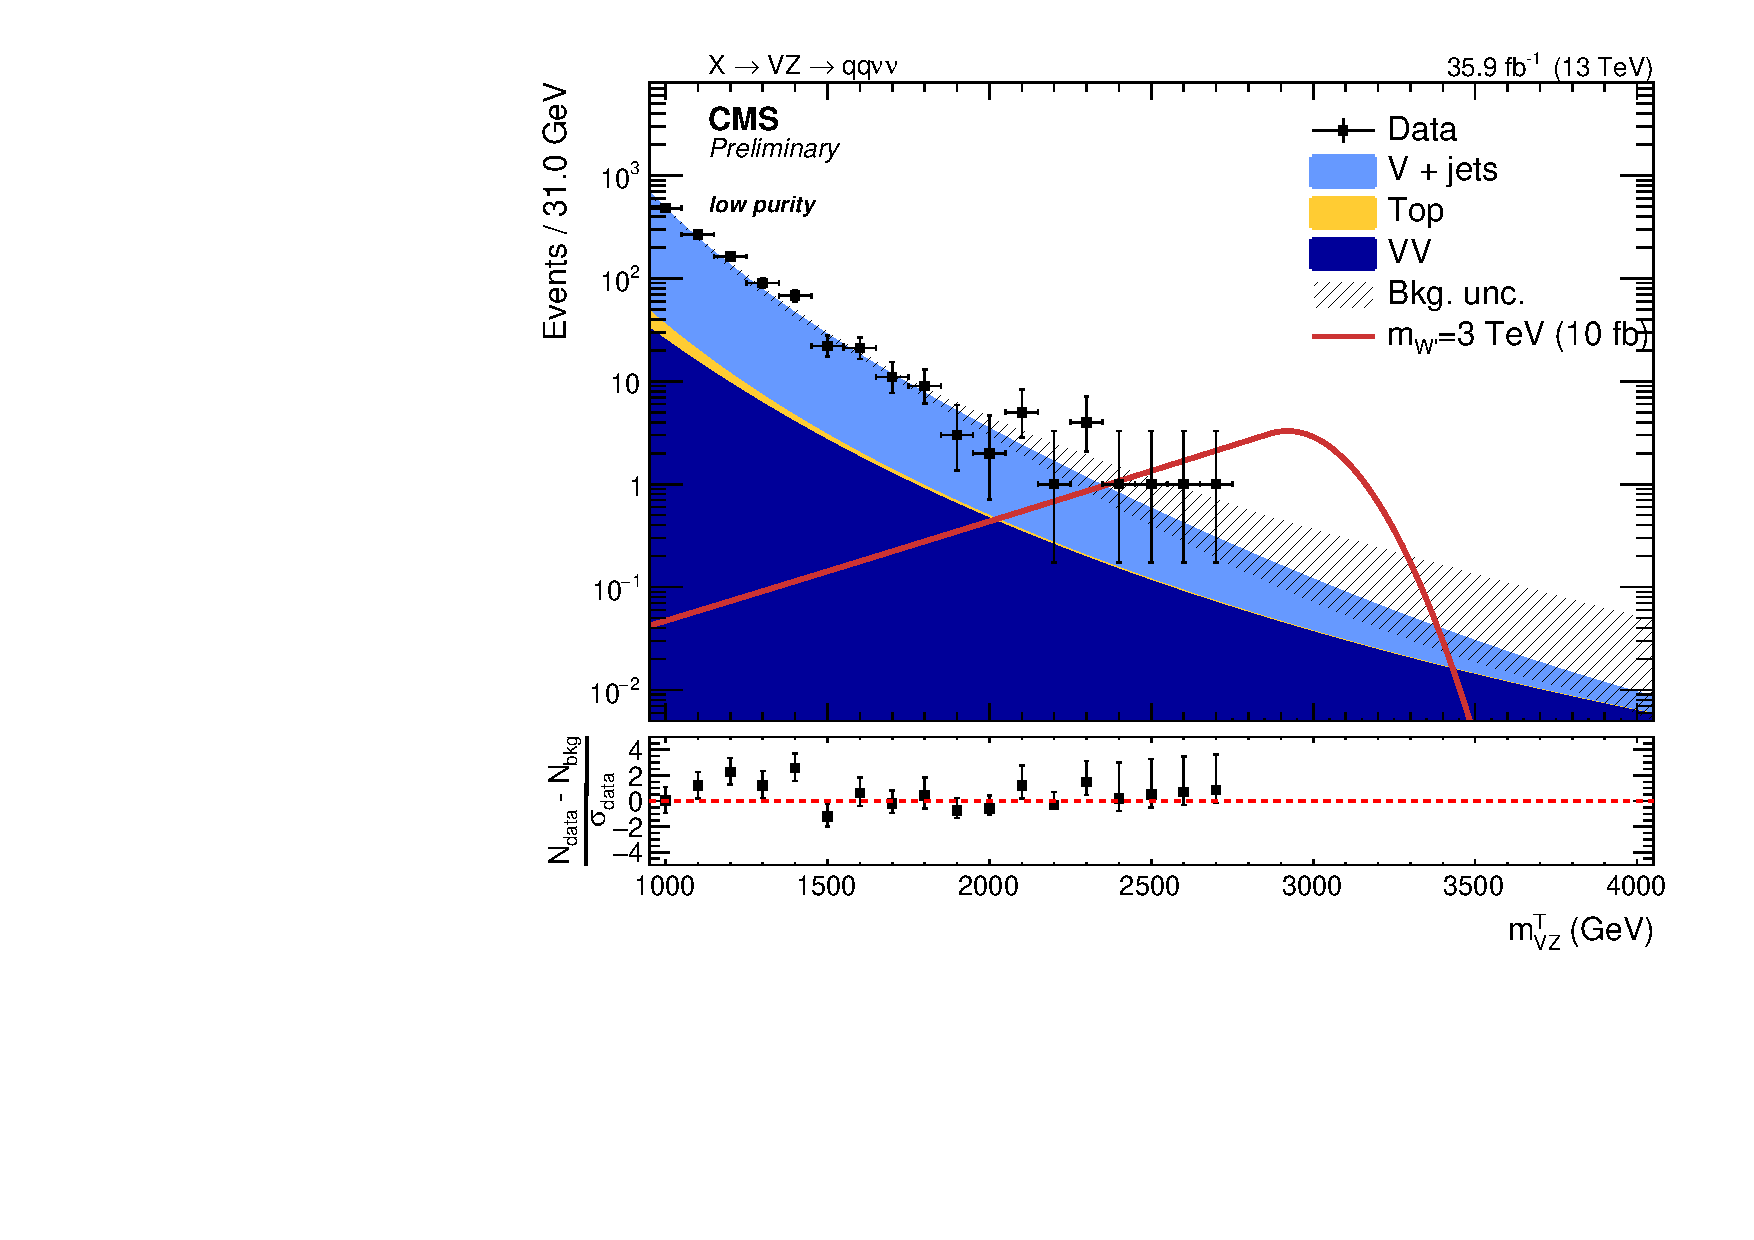
\includegraphics[width=.495\textwidth]{v9/plotsAlpha/XVZnnlp/XVZnnlp_XWZInv_BkgSR.pdf}
    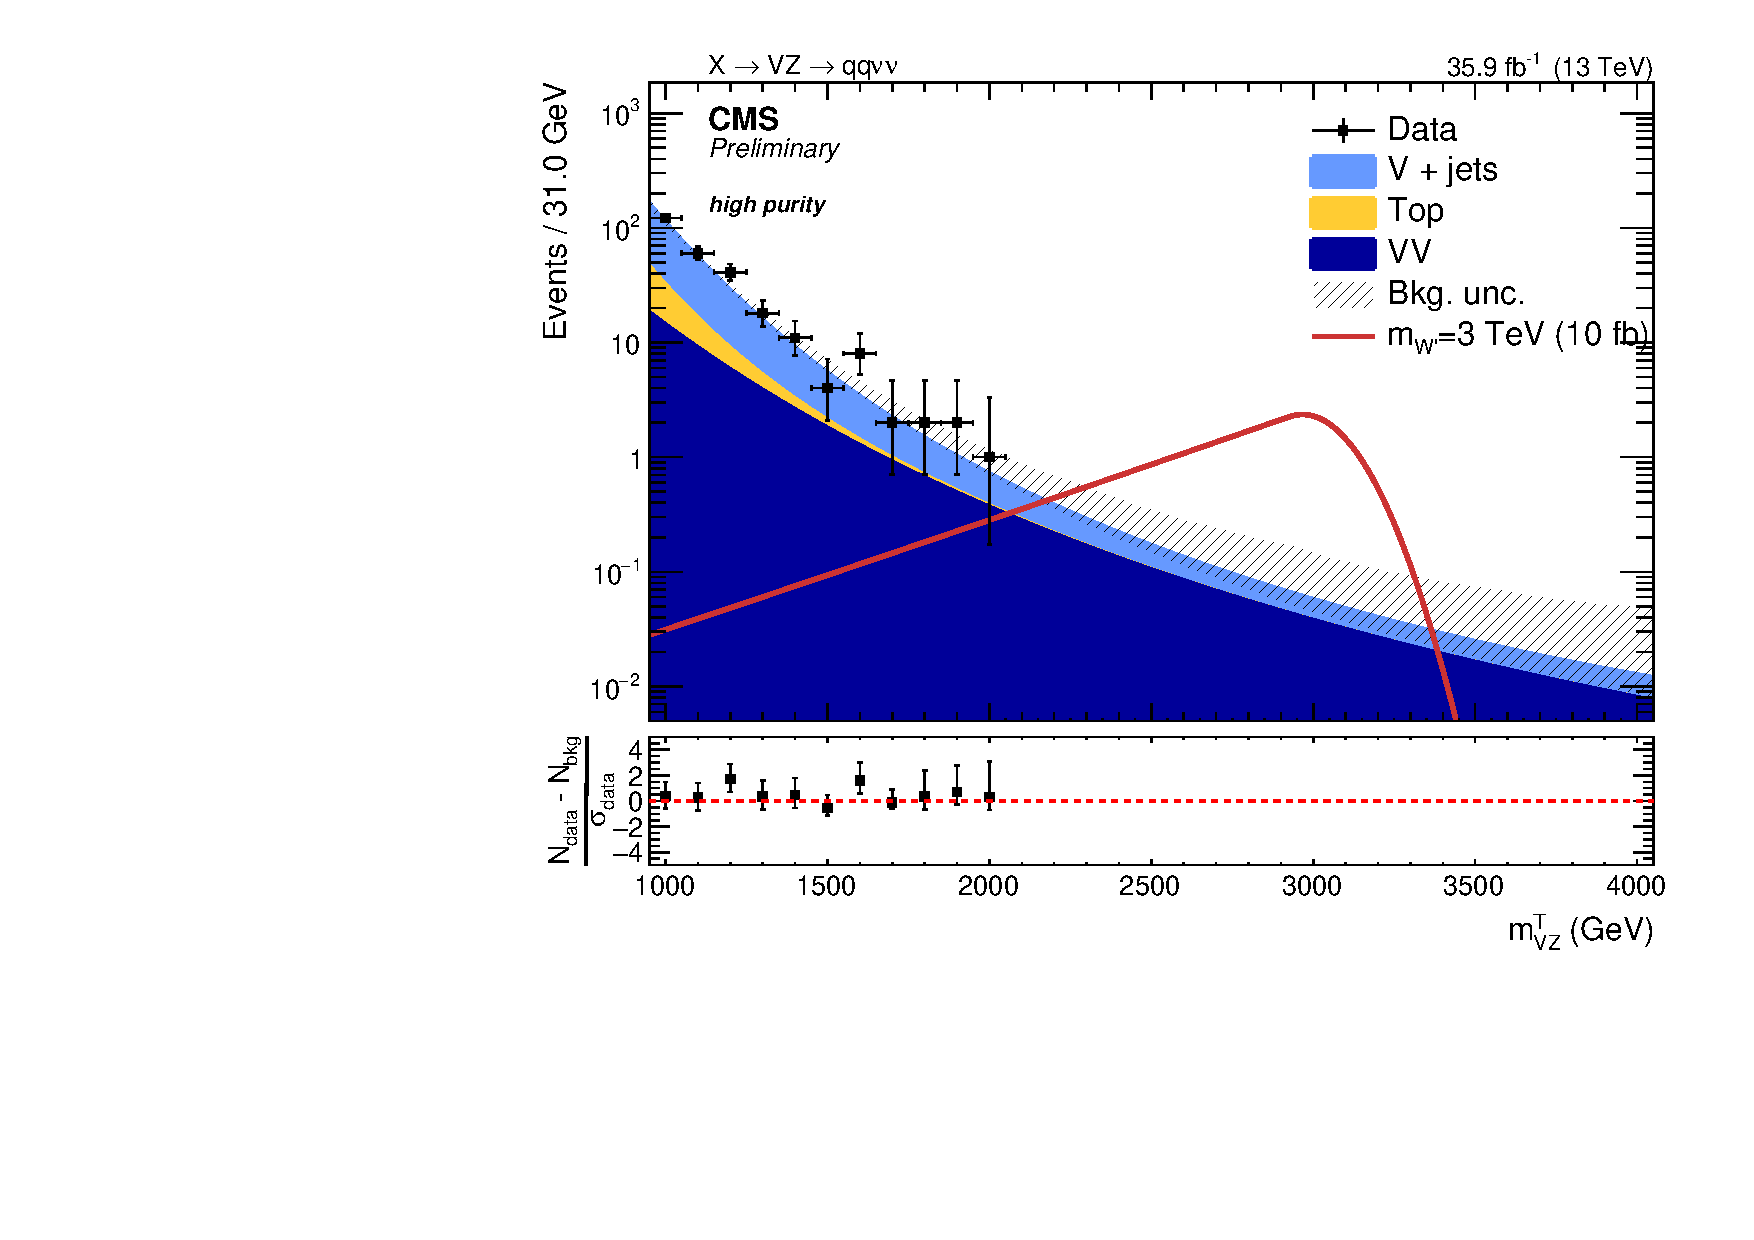
\includegraphics[width=.495\textwidth]{v9/plotsAlpha/XVZnnhp/XVZnnhp_XWZInv_BkgSR.pdf}
  \caption{Expected background predicted with the $\alpha$ method in the low- (left) and high-purity category (right), compared to observations (black markers) and a signal hypotesis of a spin-1 $W^{'}$ of mass 3 \TeV.}
  \label{fig:XVZnn_Exp}
\end{figure}

%\clearpage

\subsection{Alpha method validations}
\label{ssec:alpha_validation}


\begin{figure}[!htb]
  \centering
    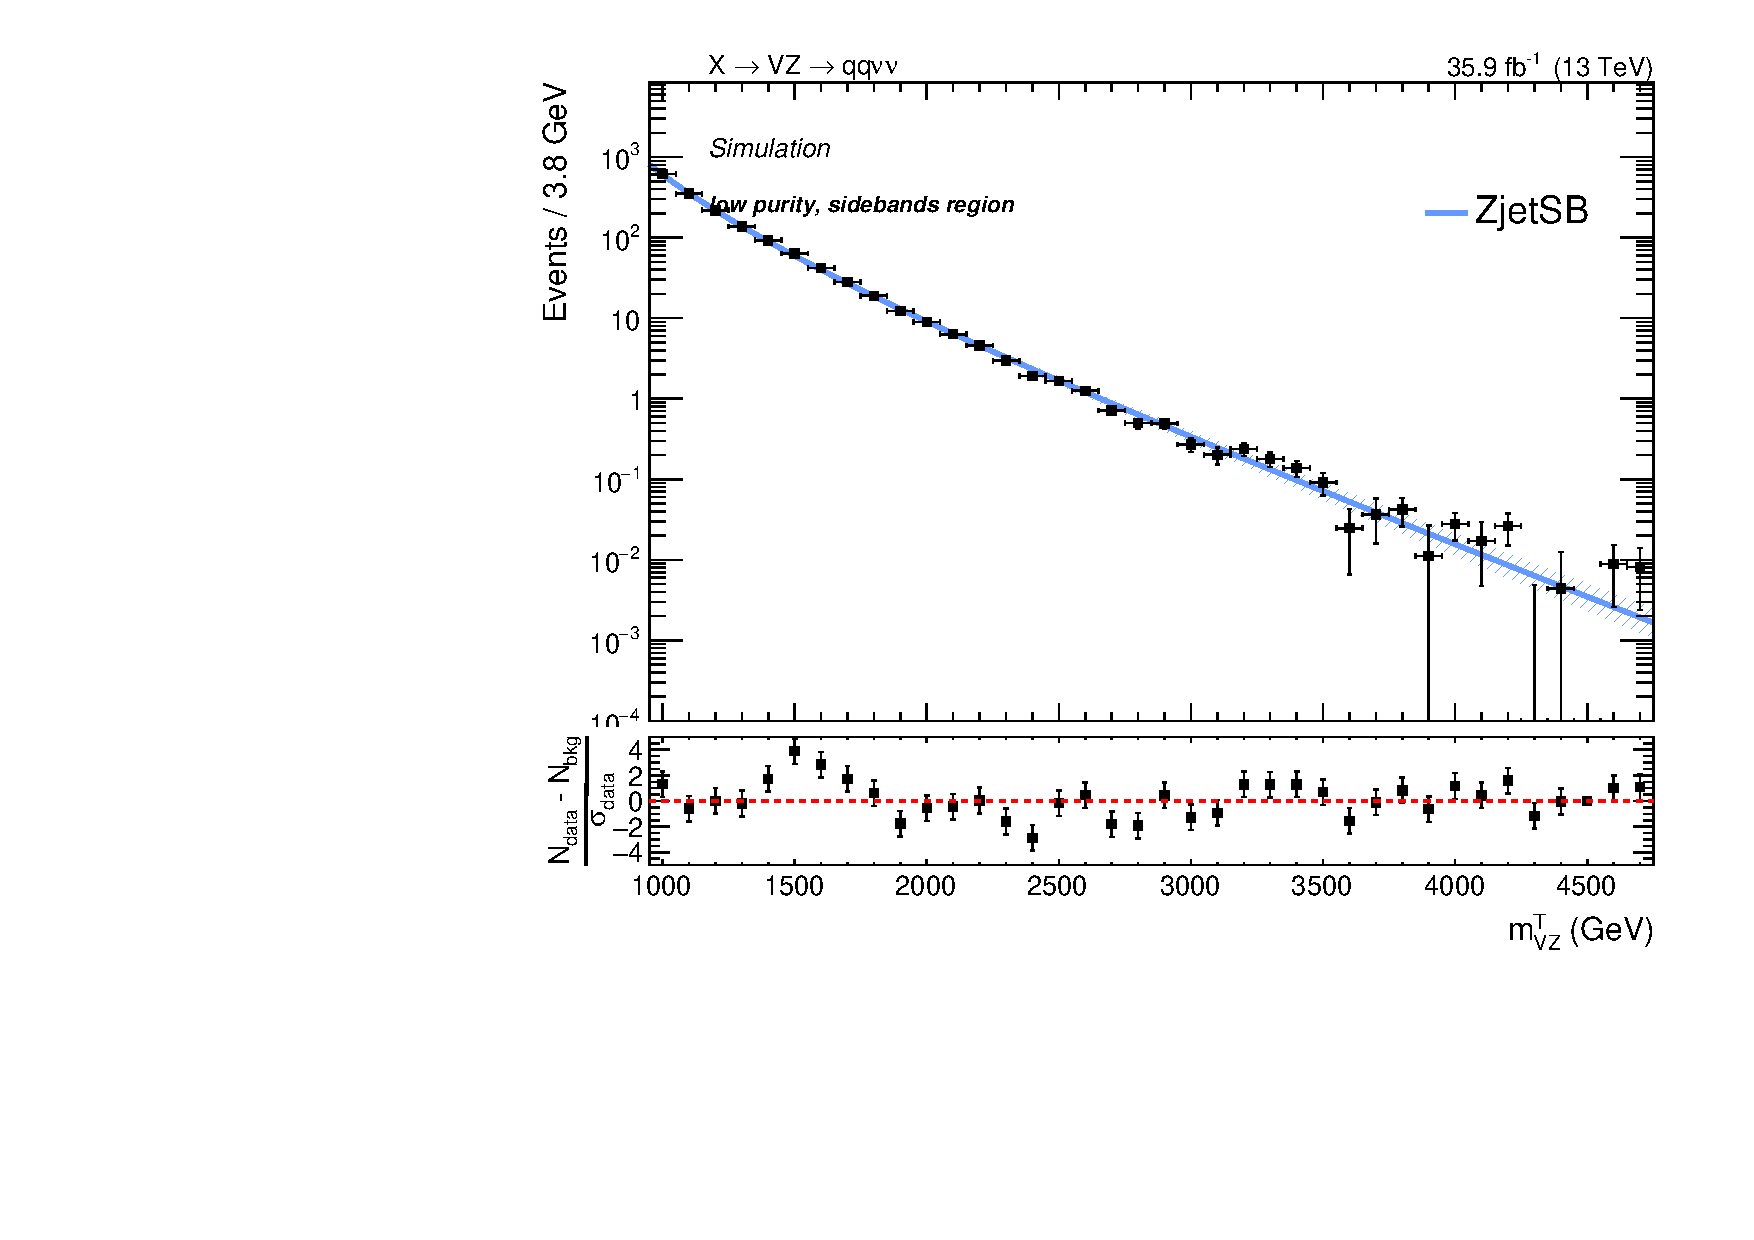
\includegraphics[width=.33\textwidth]{plotsAlpha_tesi/XVZnnlp/ZjetSB.pdf}
    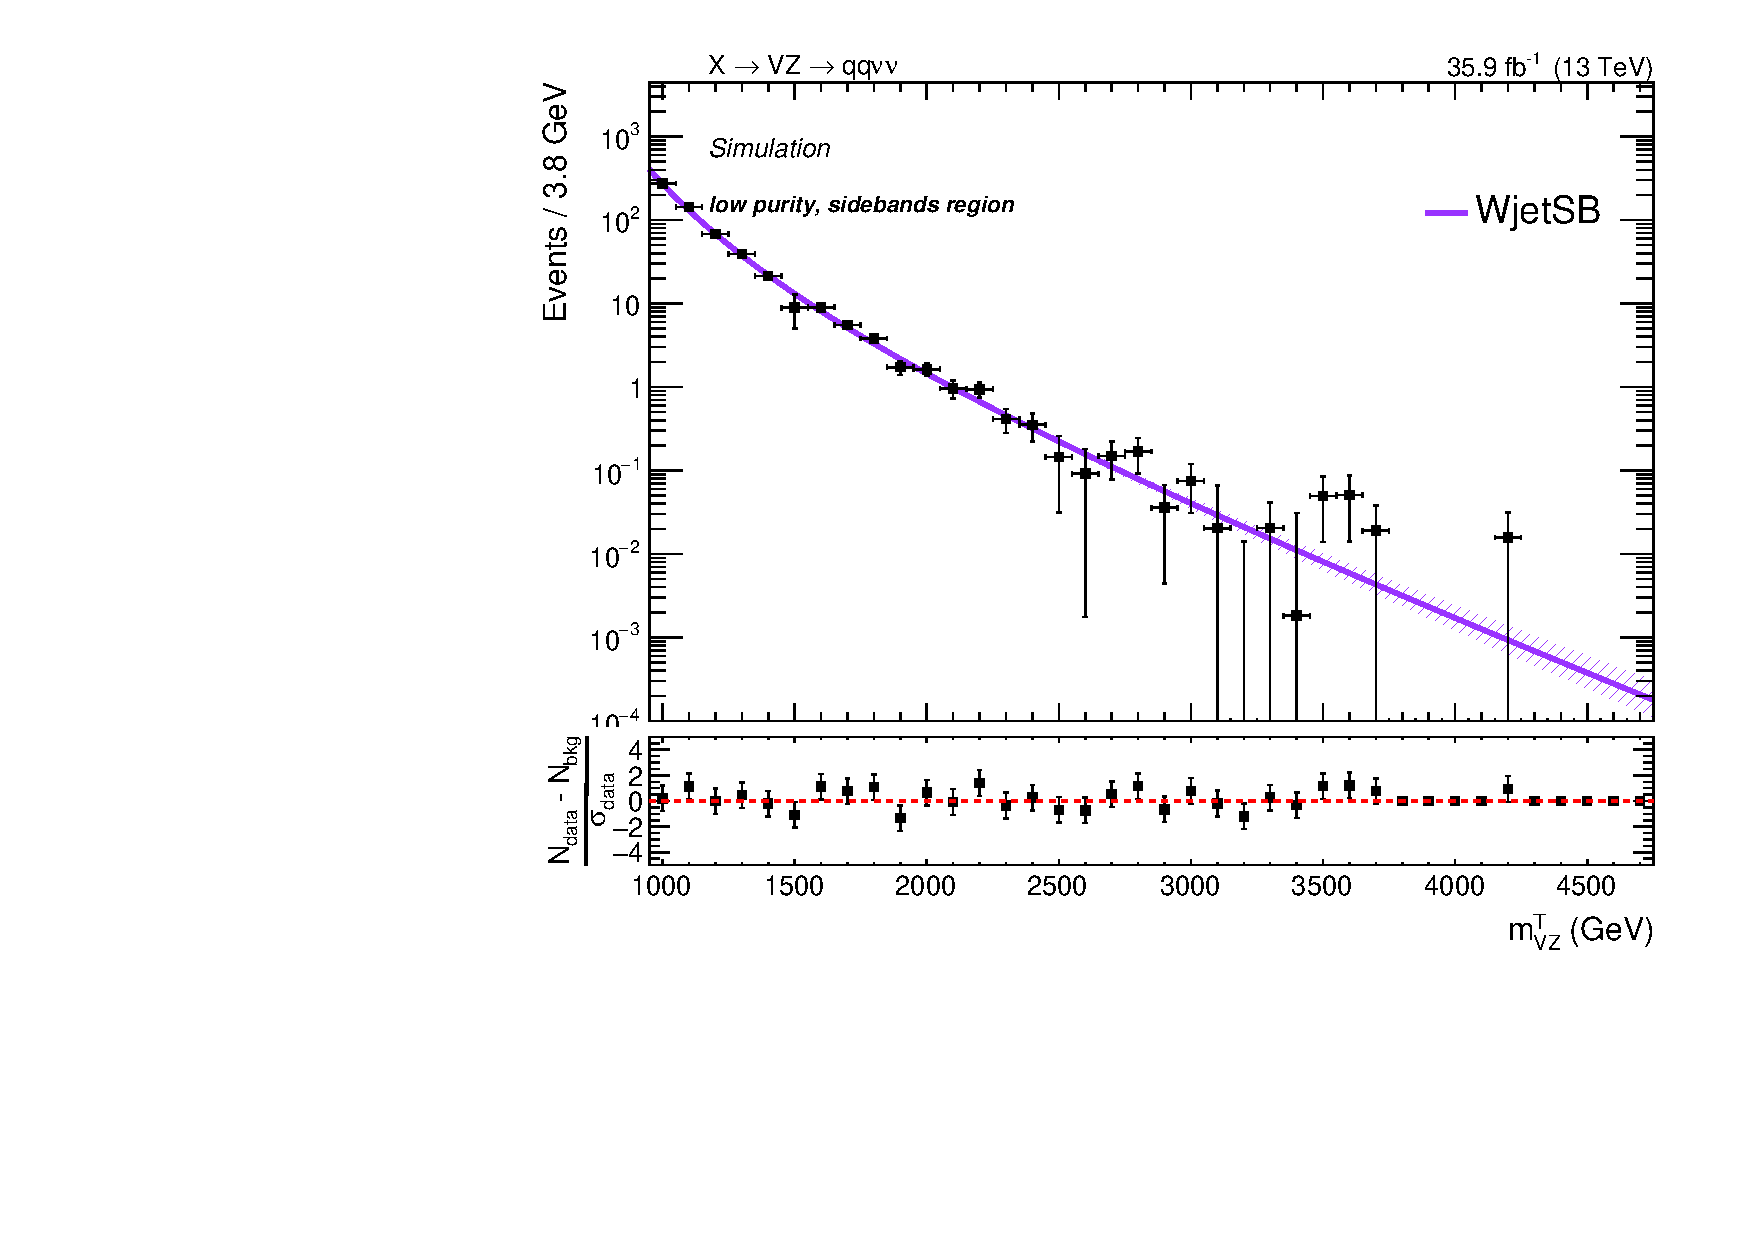
\includegraphics[width=.33\textwidth]{plotsAlpha_tesi/XVZnnlp/WjetSB.pdf}
    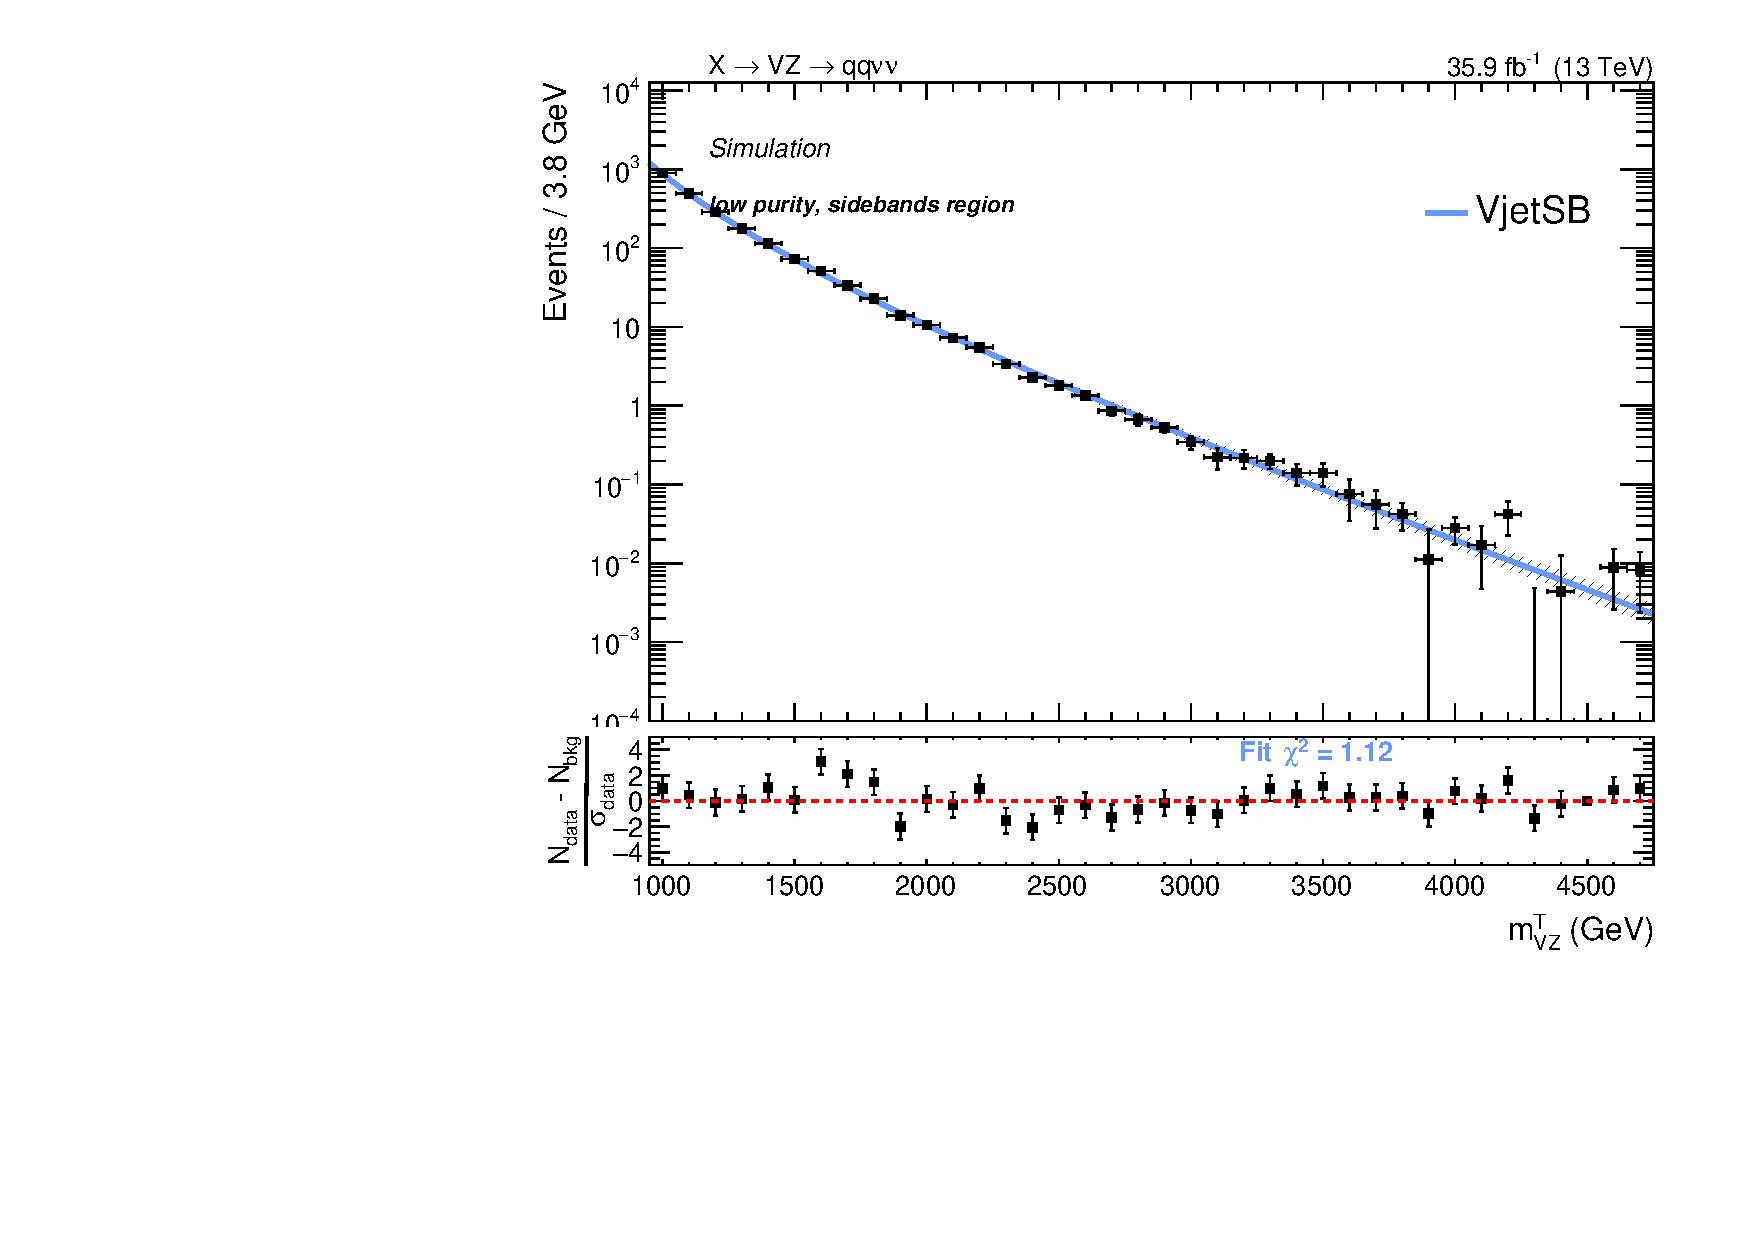
\includegraphics[width=.33\textwidth]{plotsAlpha_tesi/XVZnnlp/VjetSB.pdf}

    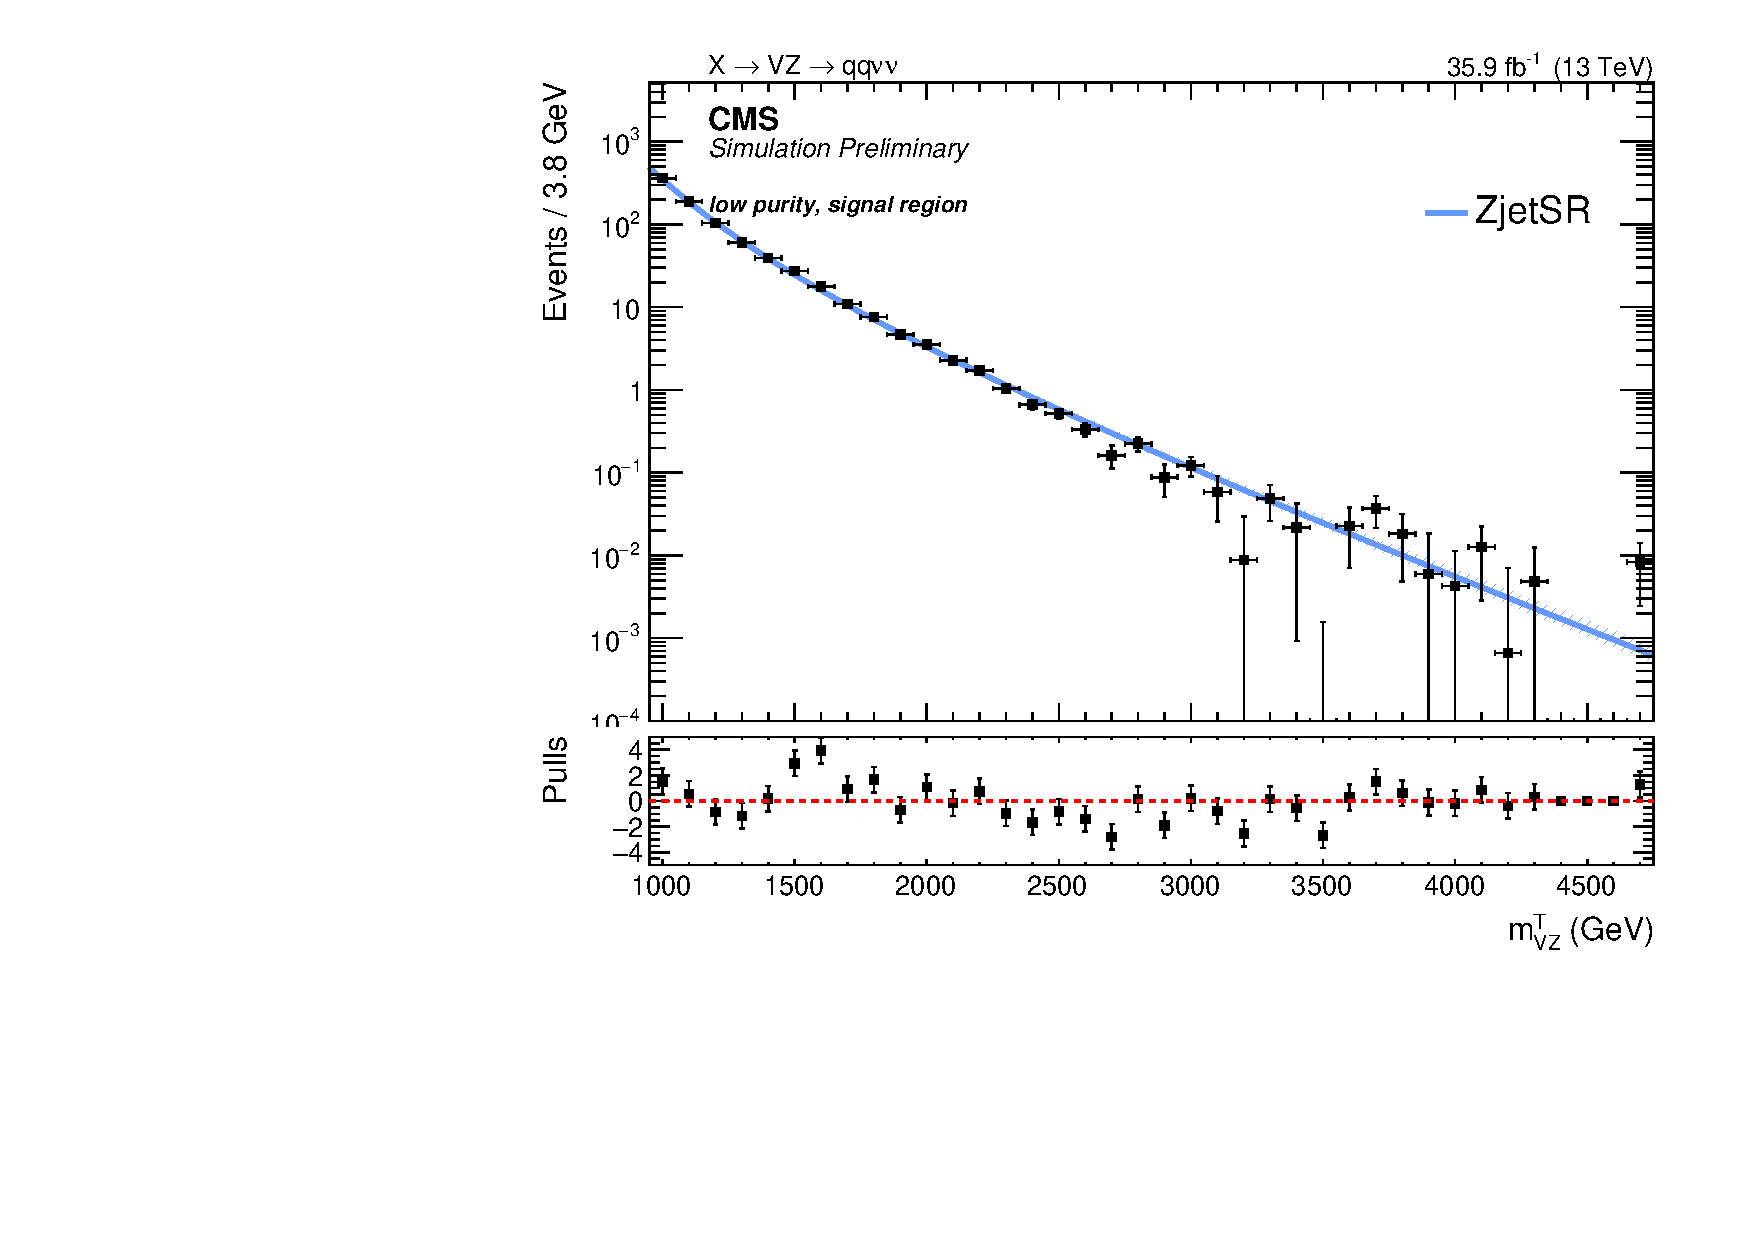
\includegraphics[width=.33\textwidth]{plotsAlpha_tesi/XVZnnlp/ZjetSR.pdf}
    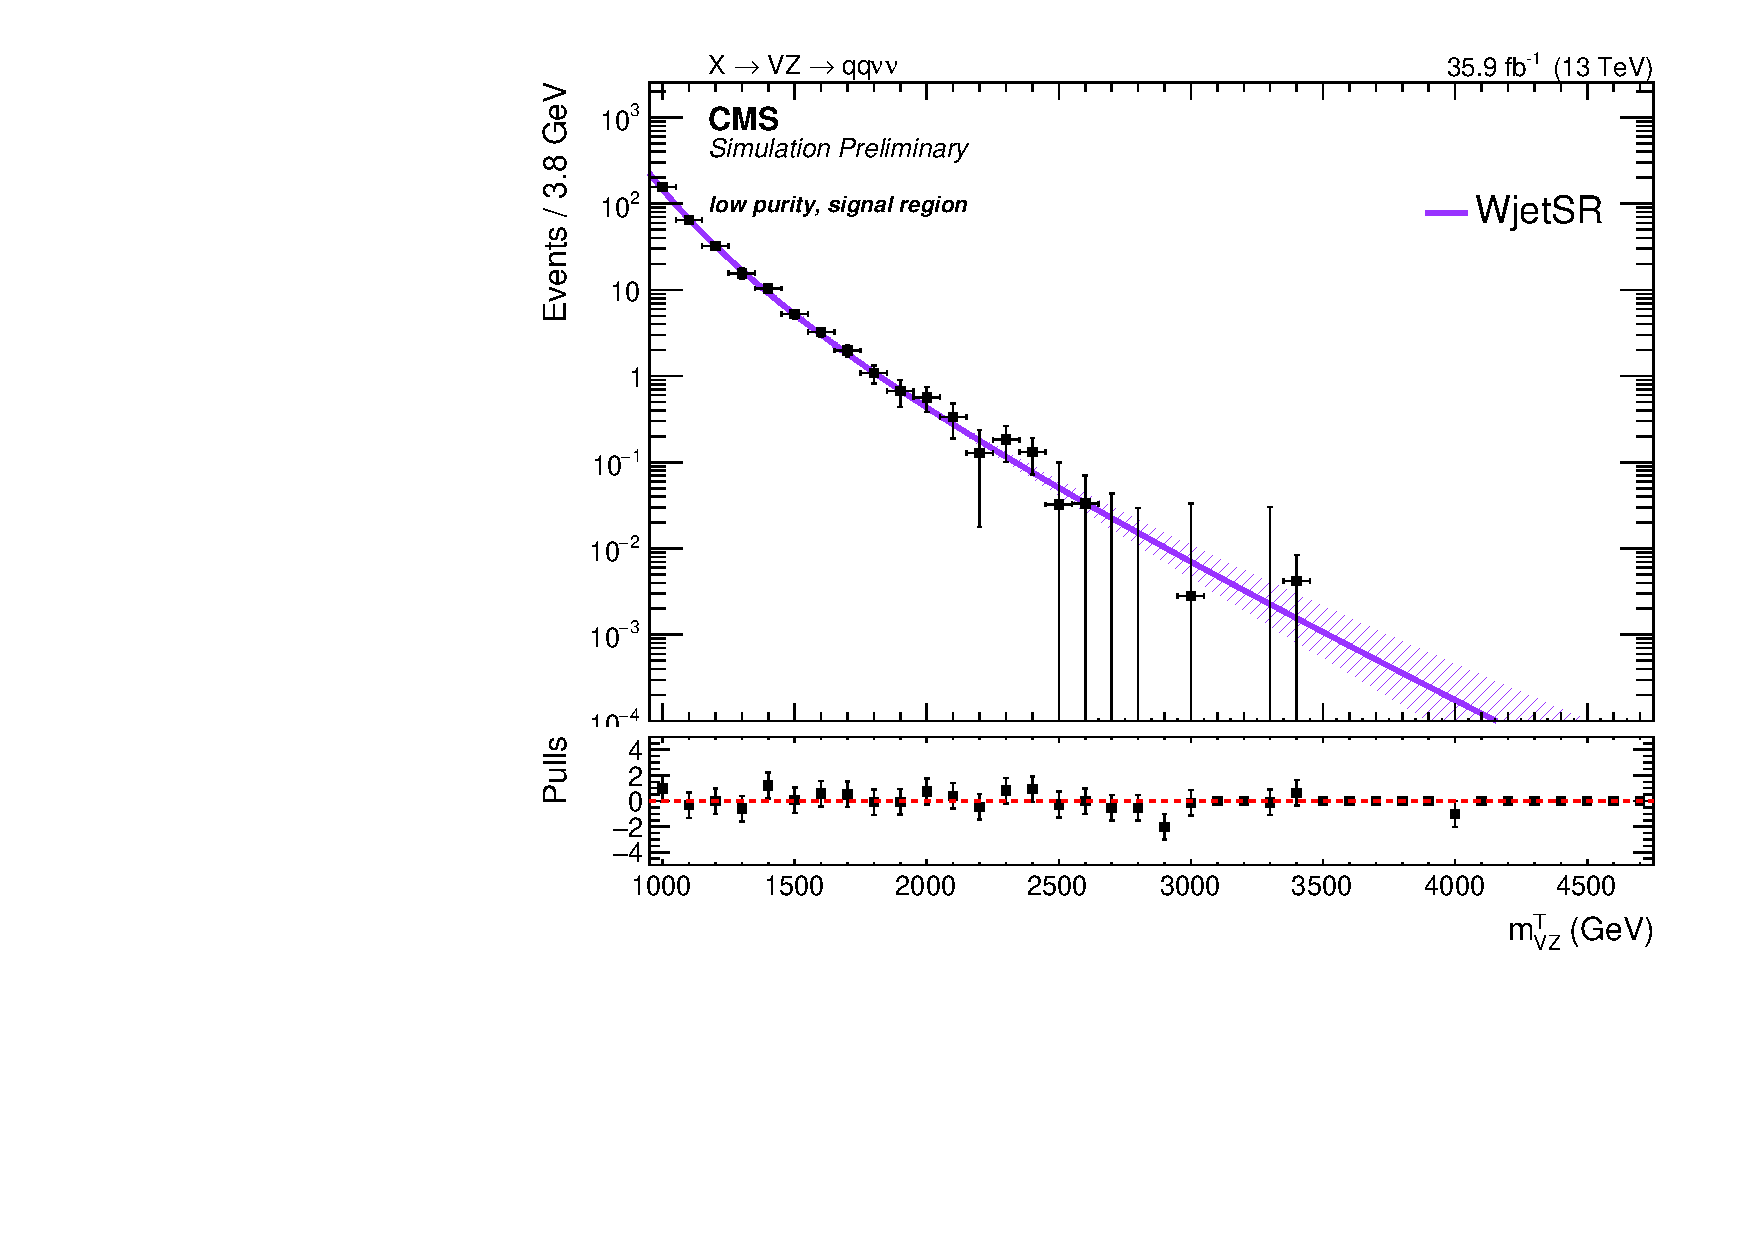
\includegraphics[width=.33\textwidth]{plotsAlpha_tesi/XVZnnlp/WjetSR.pdf}
    \includegraphics[width=.33\textwidth]{plotsAlpha_tesi/XVZnnlp/VjetSR.pdf}

  \caption{Validation of the $\alpha$ method, low-purity category. Top: fits to the simulated background components \Z + jets (left), \W + jets (center), and their combination \V + jets (right), in the sidebands (SB). Bottom: fits to the simulated background components \Z + jets (left), \W + jets (center), and their combination \V + jets (right), in the signal region.}
  \label{fig:XVZnnlp_WZvalidation}
\end{figure}

\begin{figure}[!htb]
  \centering
    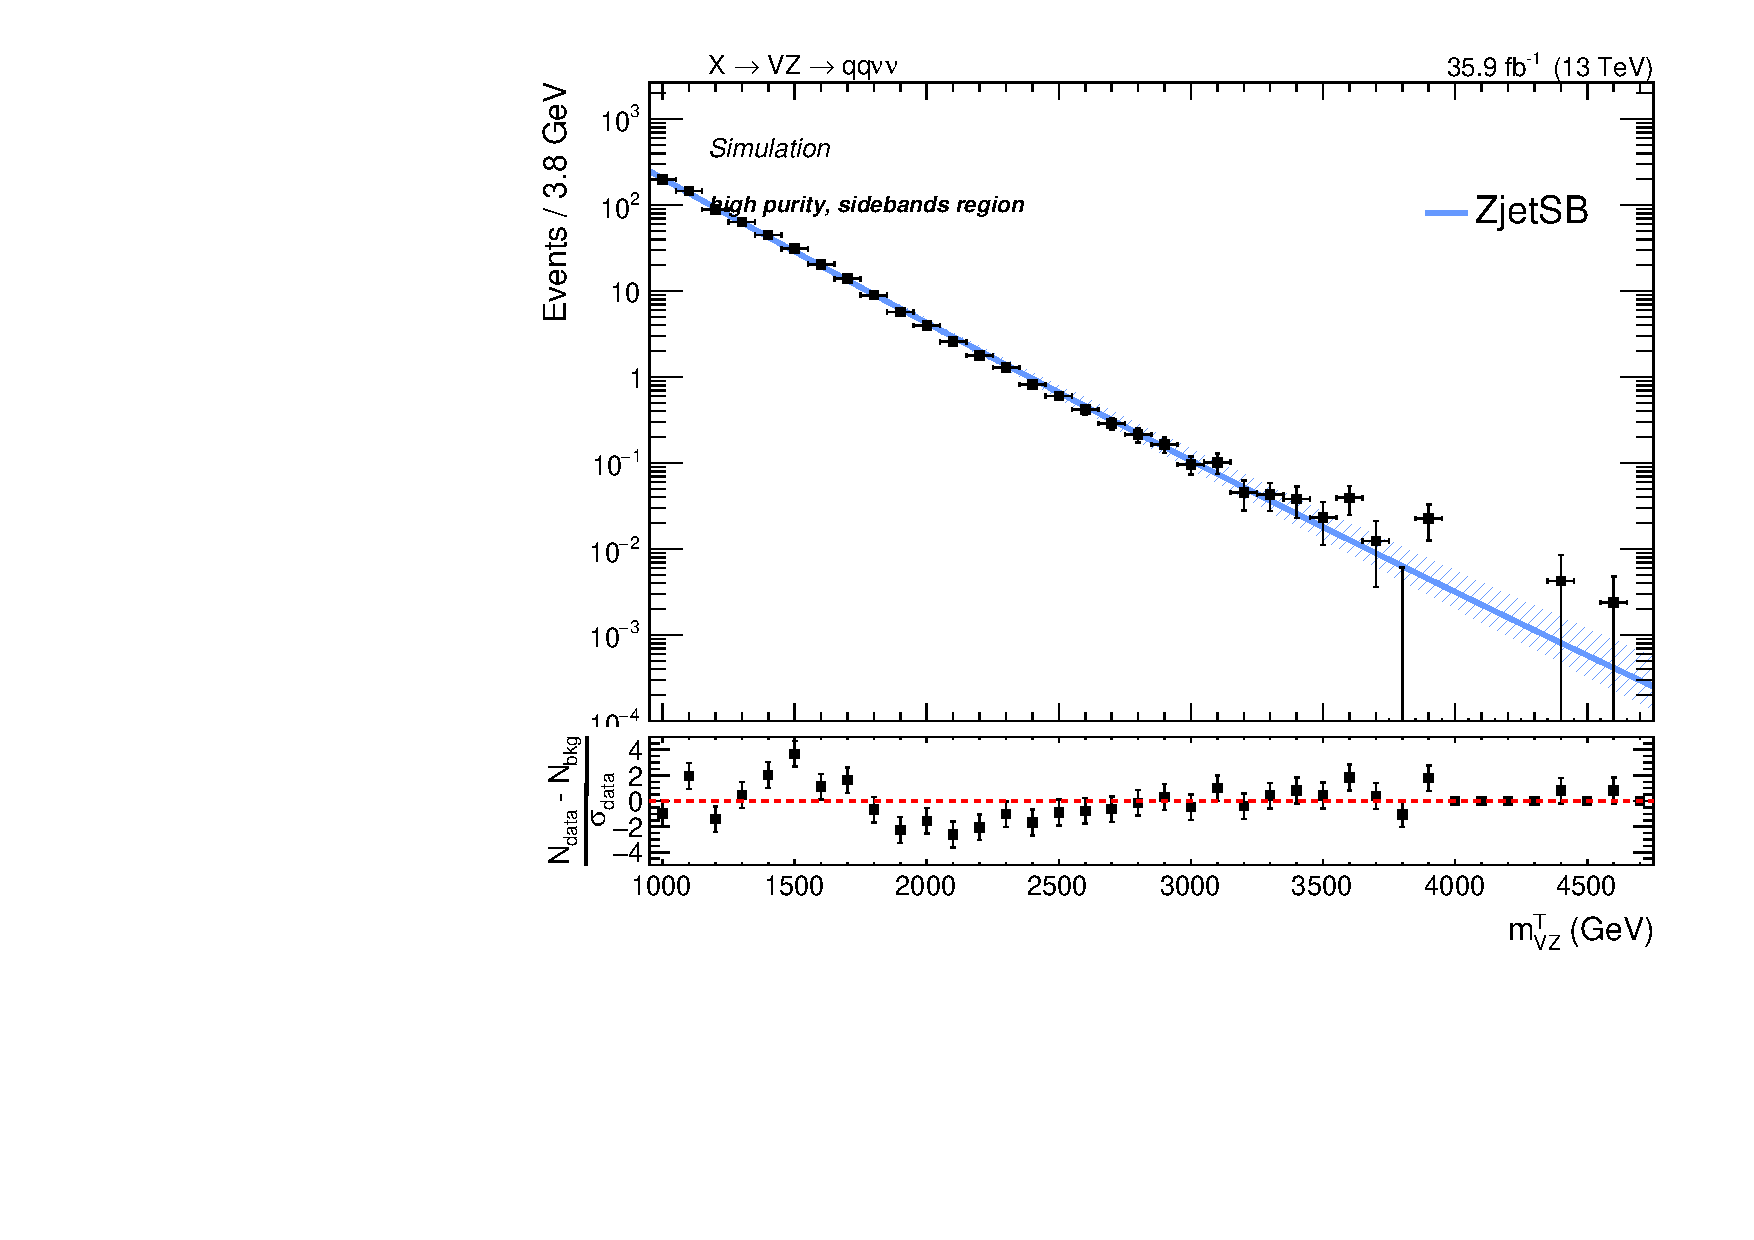
\includegraphics[width=.33\textwidth]{plotsAlpha_tesi/XVZnnhp/ZjetSB.pdf}
    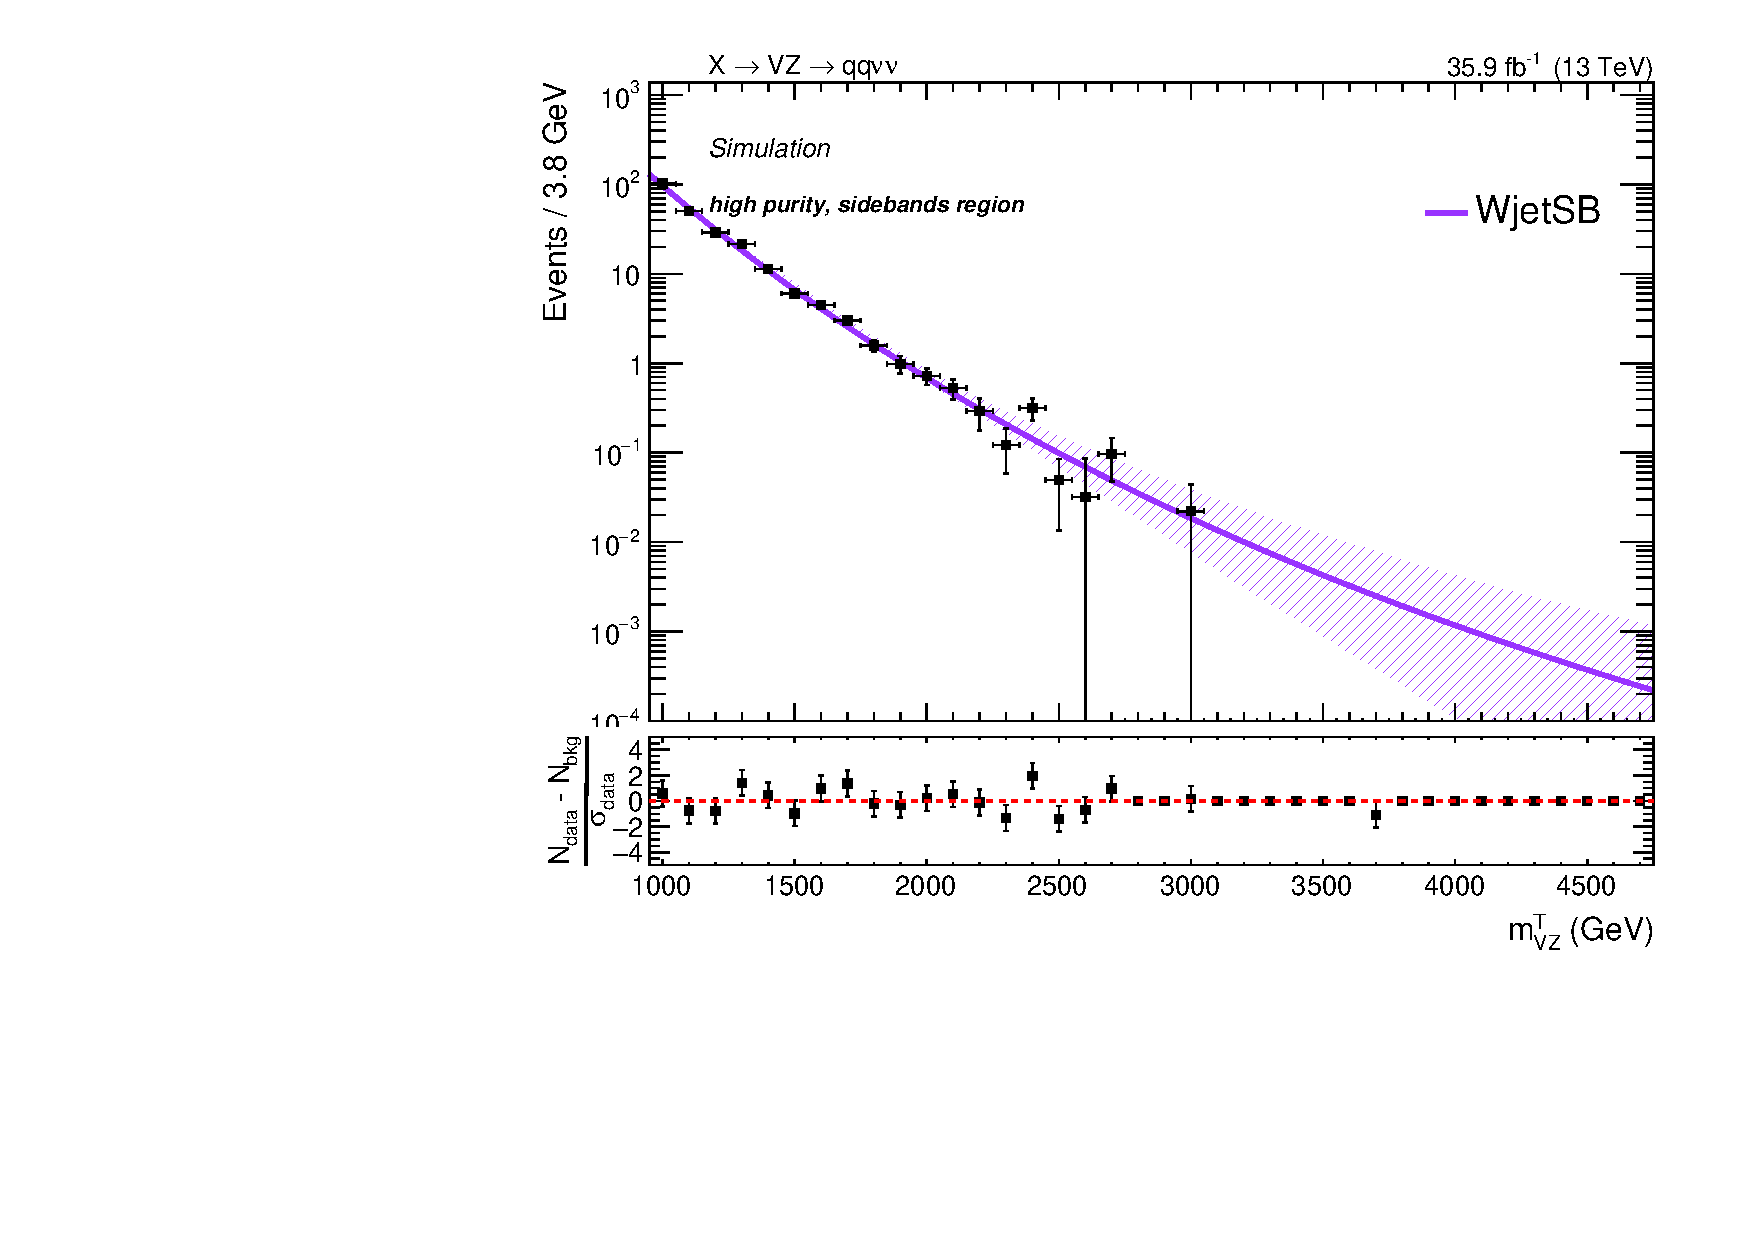
\includegraphics[width=.33\textwidth]{plotsAlpha_tesi/XVZnnhp/WjetSB.pdf}
    \includegraphics[width=.33\textwidth]{plotsAlpha_tesi/XVZnnhp/VjetSB.pdf}

    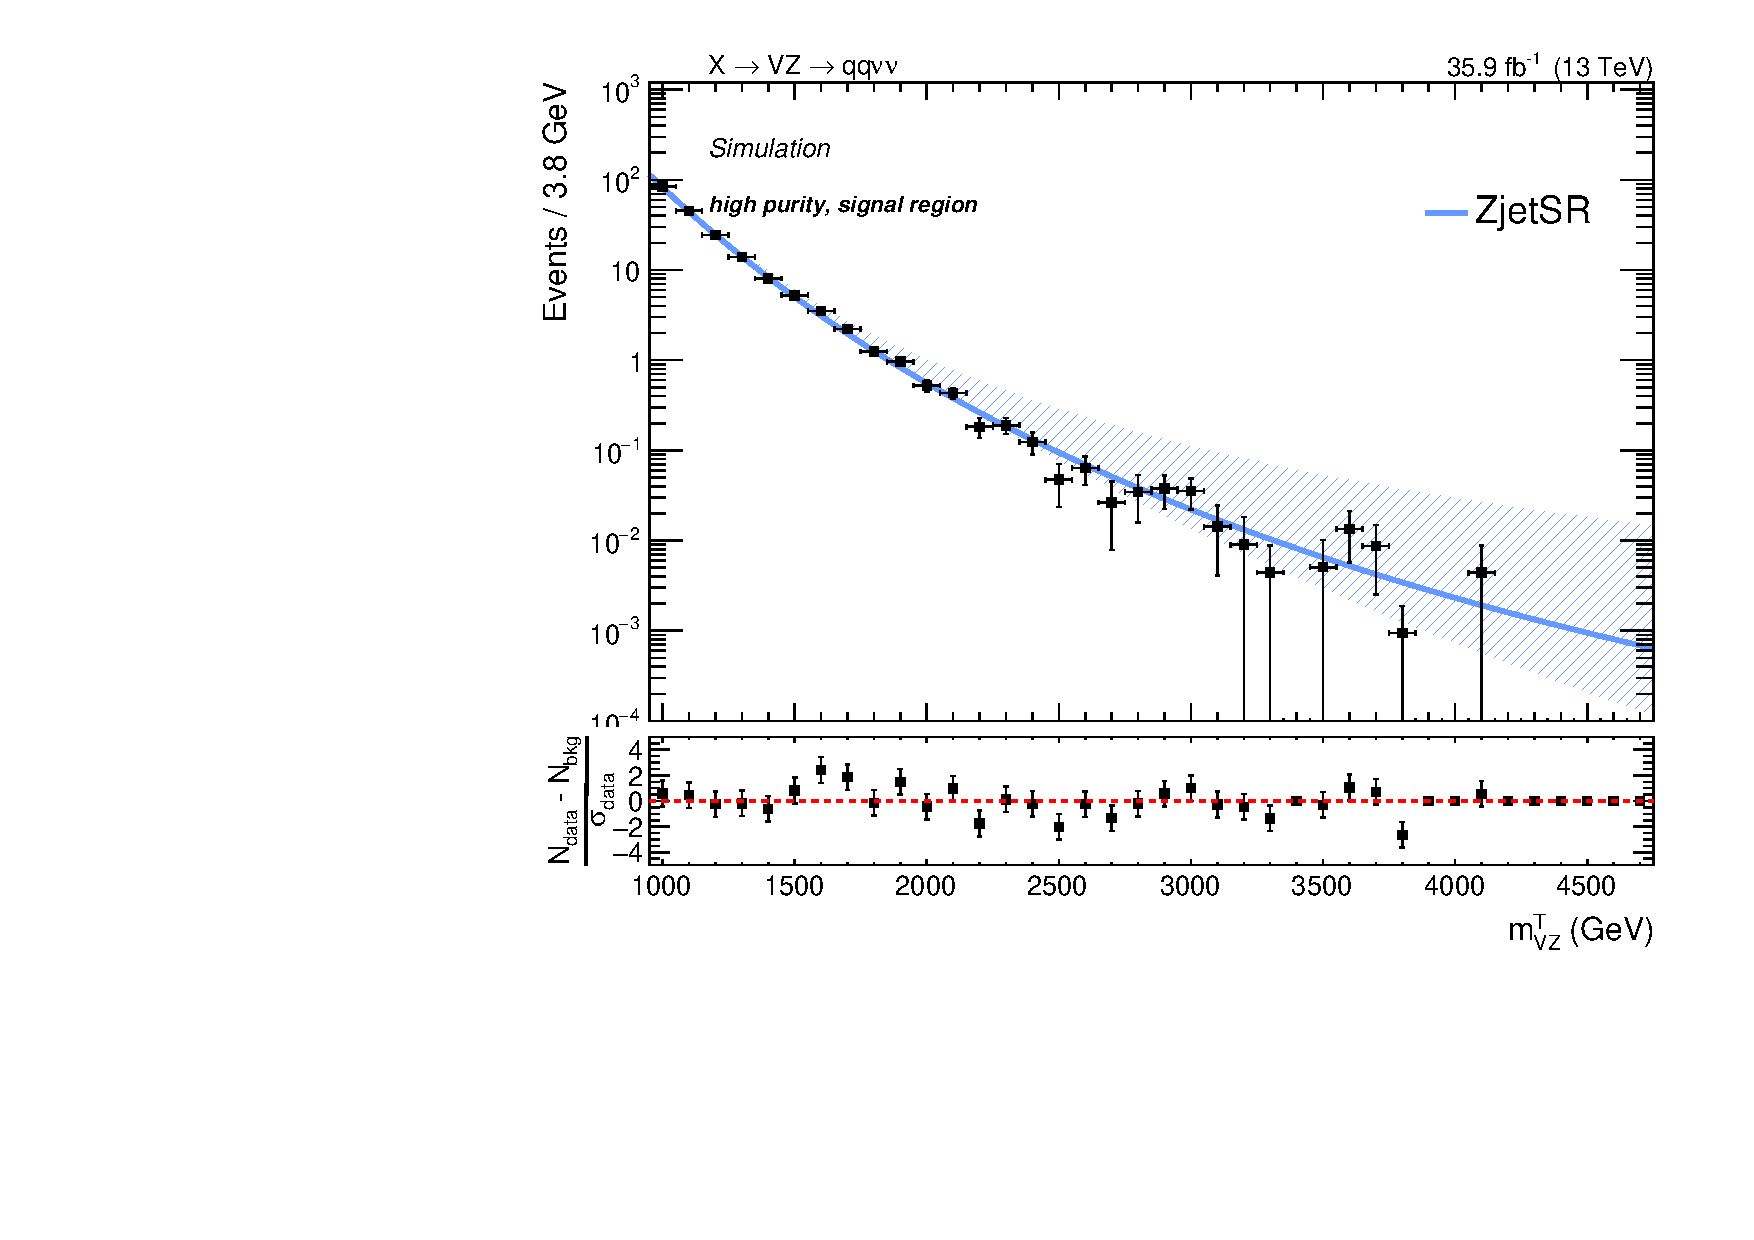
\includegraphics[width=.33\textwidth]{plotsAlpha_tesi/XVZnnhp/ZjetSR.pdf}
    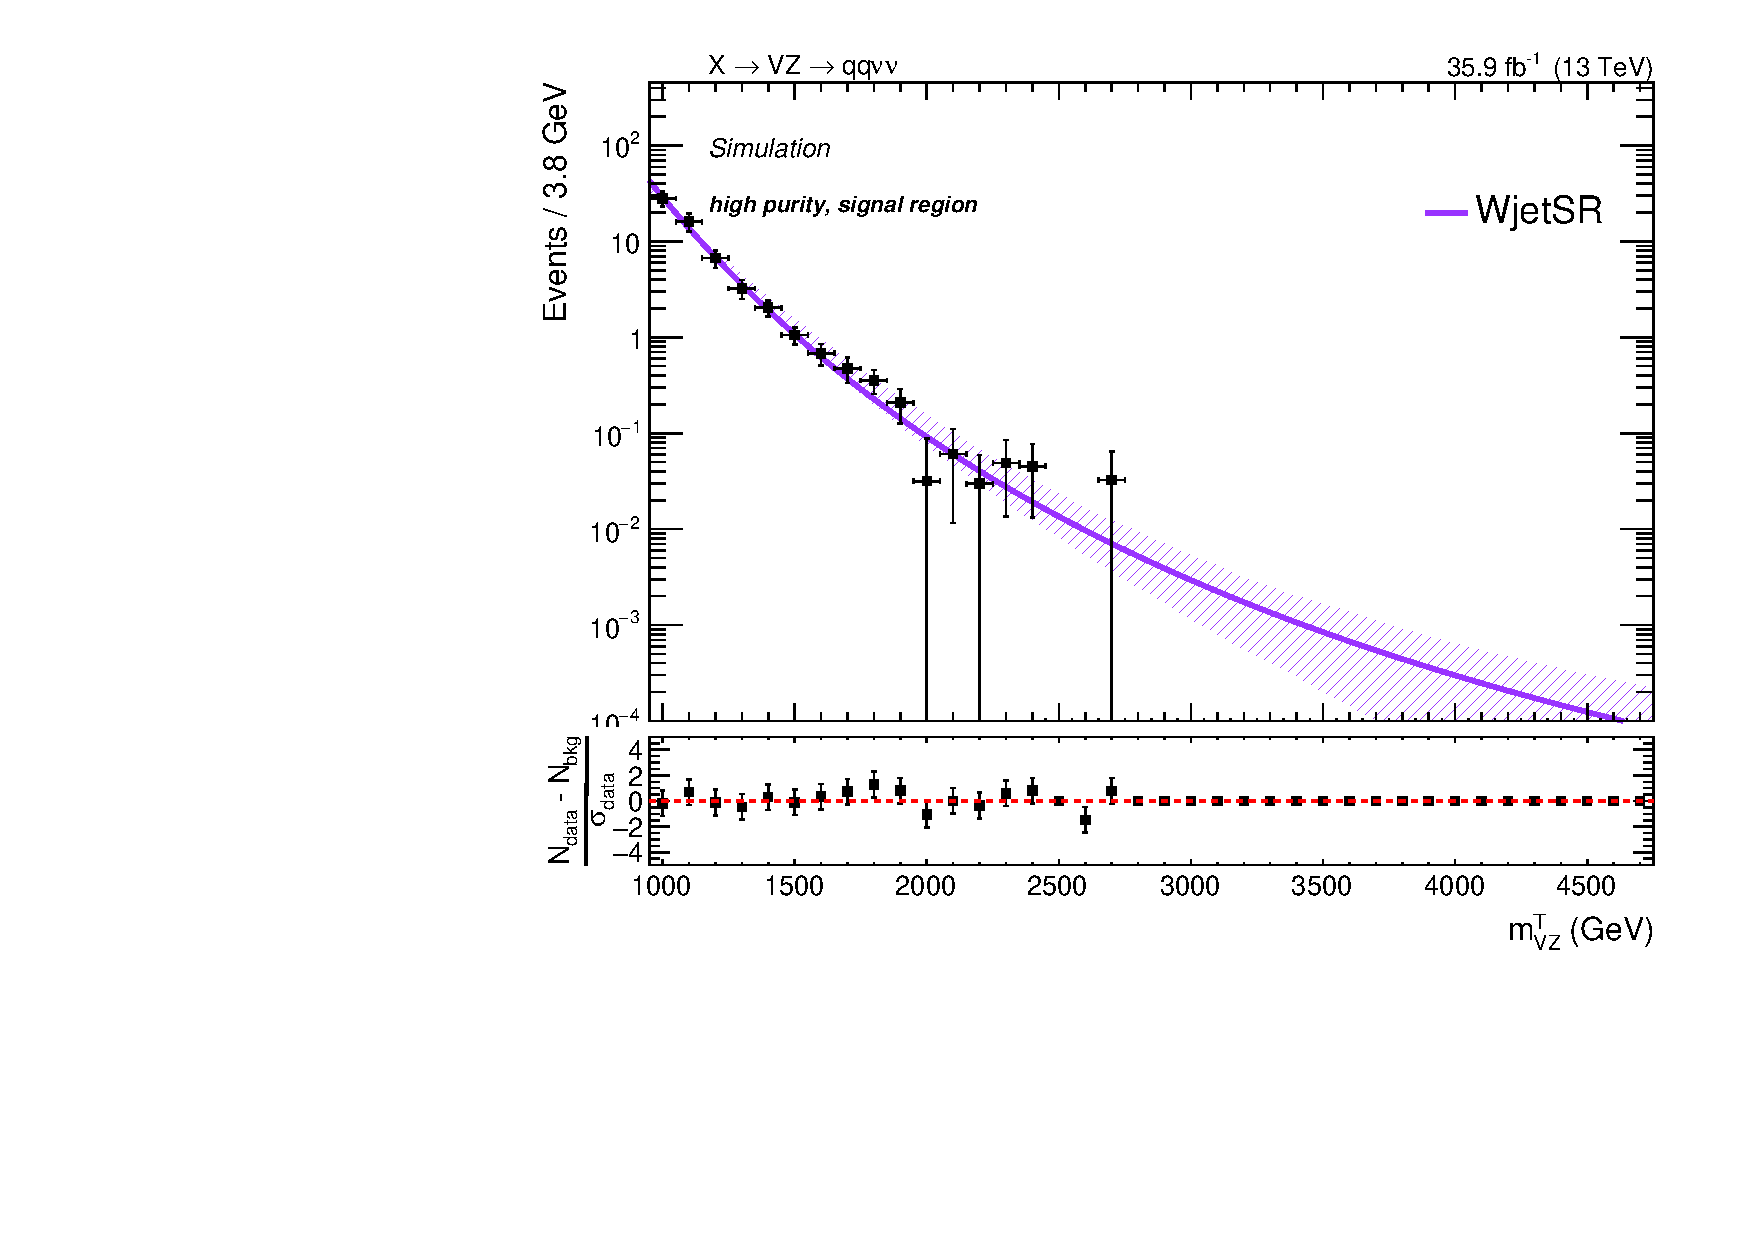
\includegraphics[width=.33\textwidth]{plotsAlpha_tesi/XVZnnhp/WjetSR.pdf}
    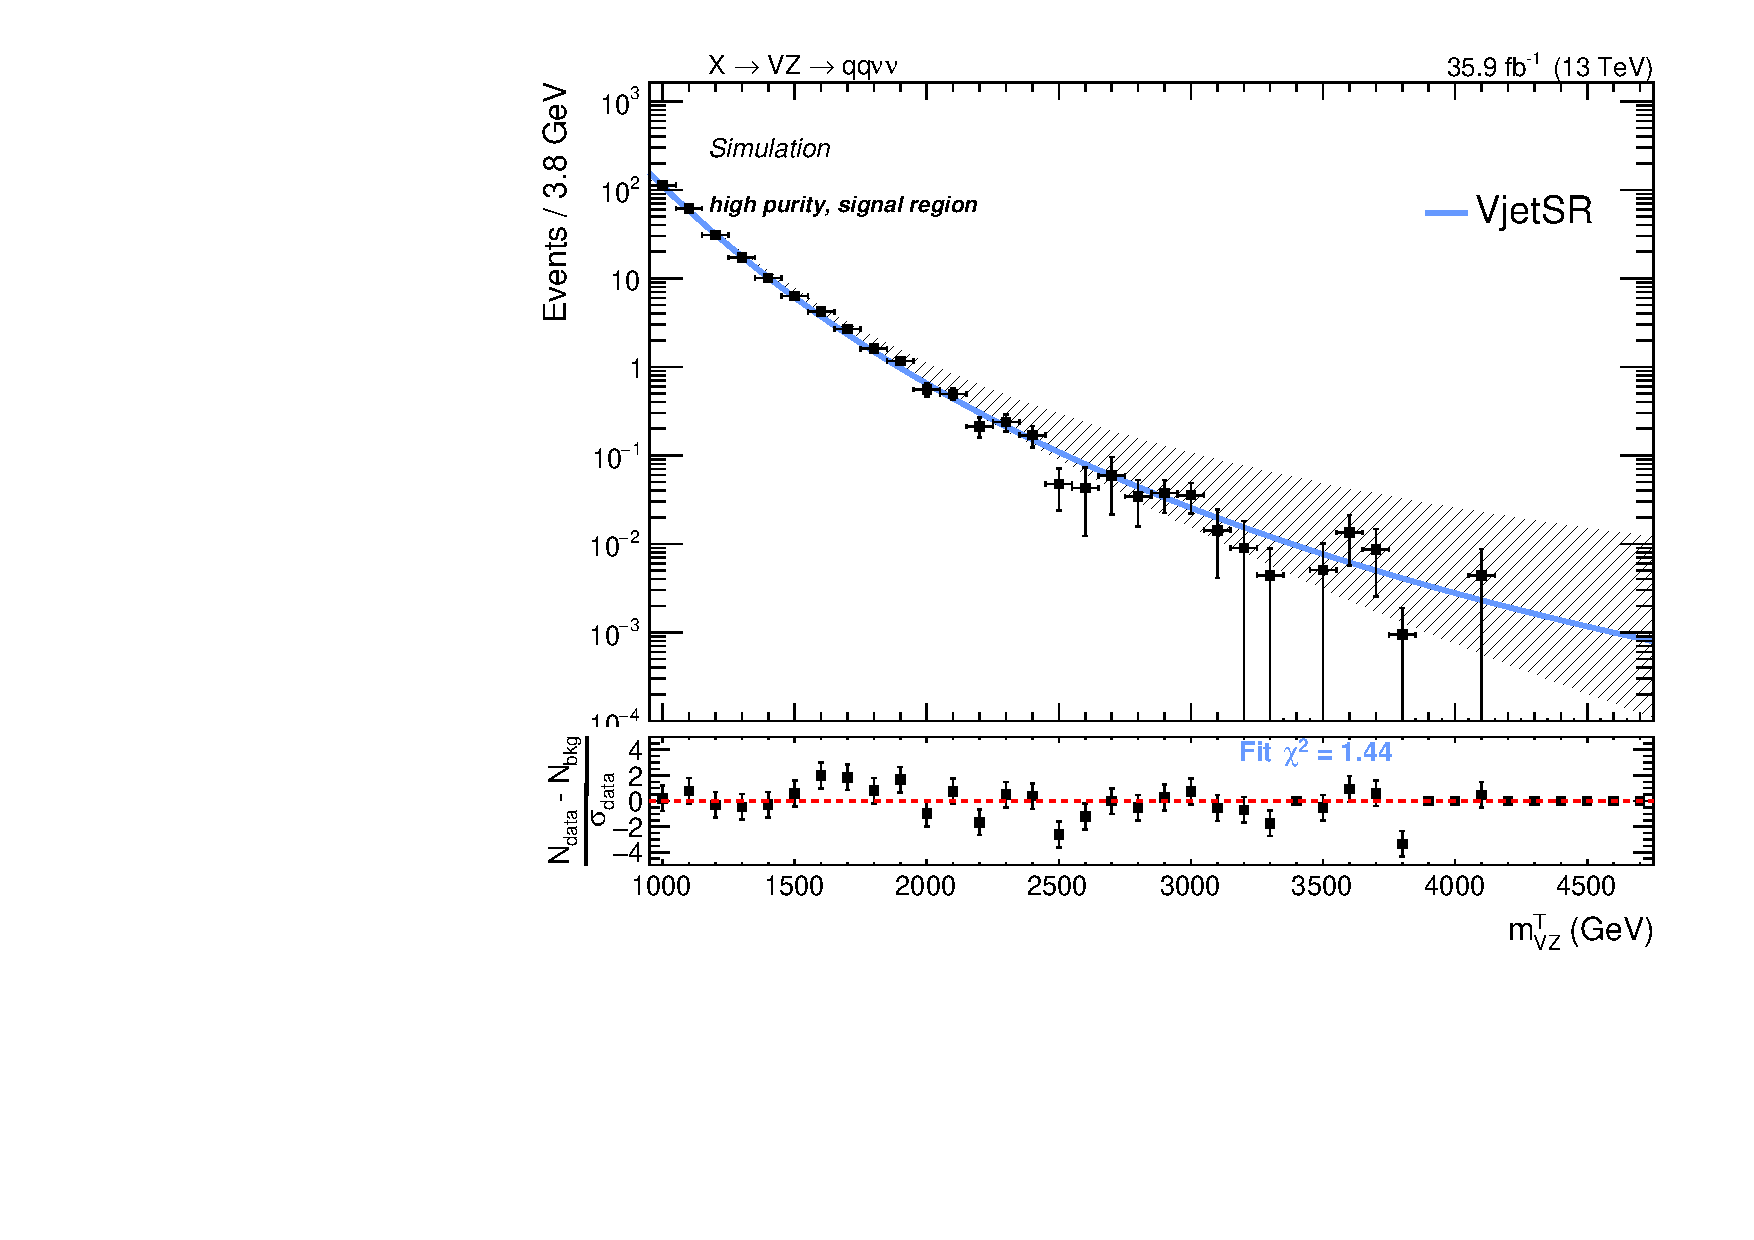
\includegraphics[width=.33\textwidth]{plotsAlpha_tesi/XVZnnhp/VjetSR.pdf}

  \caption{Validation of the $\alpha$ method, high-purity category. Top: fits to the simulated background components \Z + jets (left), \W + jets (center), and their combination \V + jets (right), in the sidebands (SB). Bottom: fits to the simulated background components \Z + jets (left), \W + jets (center), and their combination \V + jets (right), in the signal region.}
  \label{fig:XVZnnhp_WZvalidation}
\end{figure}

\begin{figure}[!htb]
  \centering
    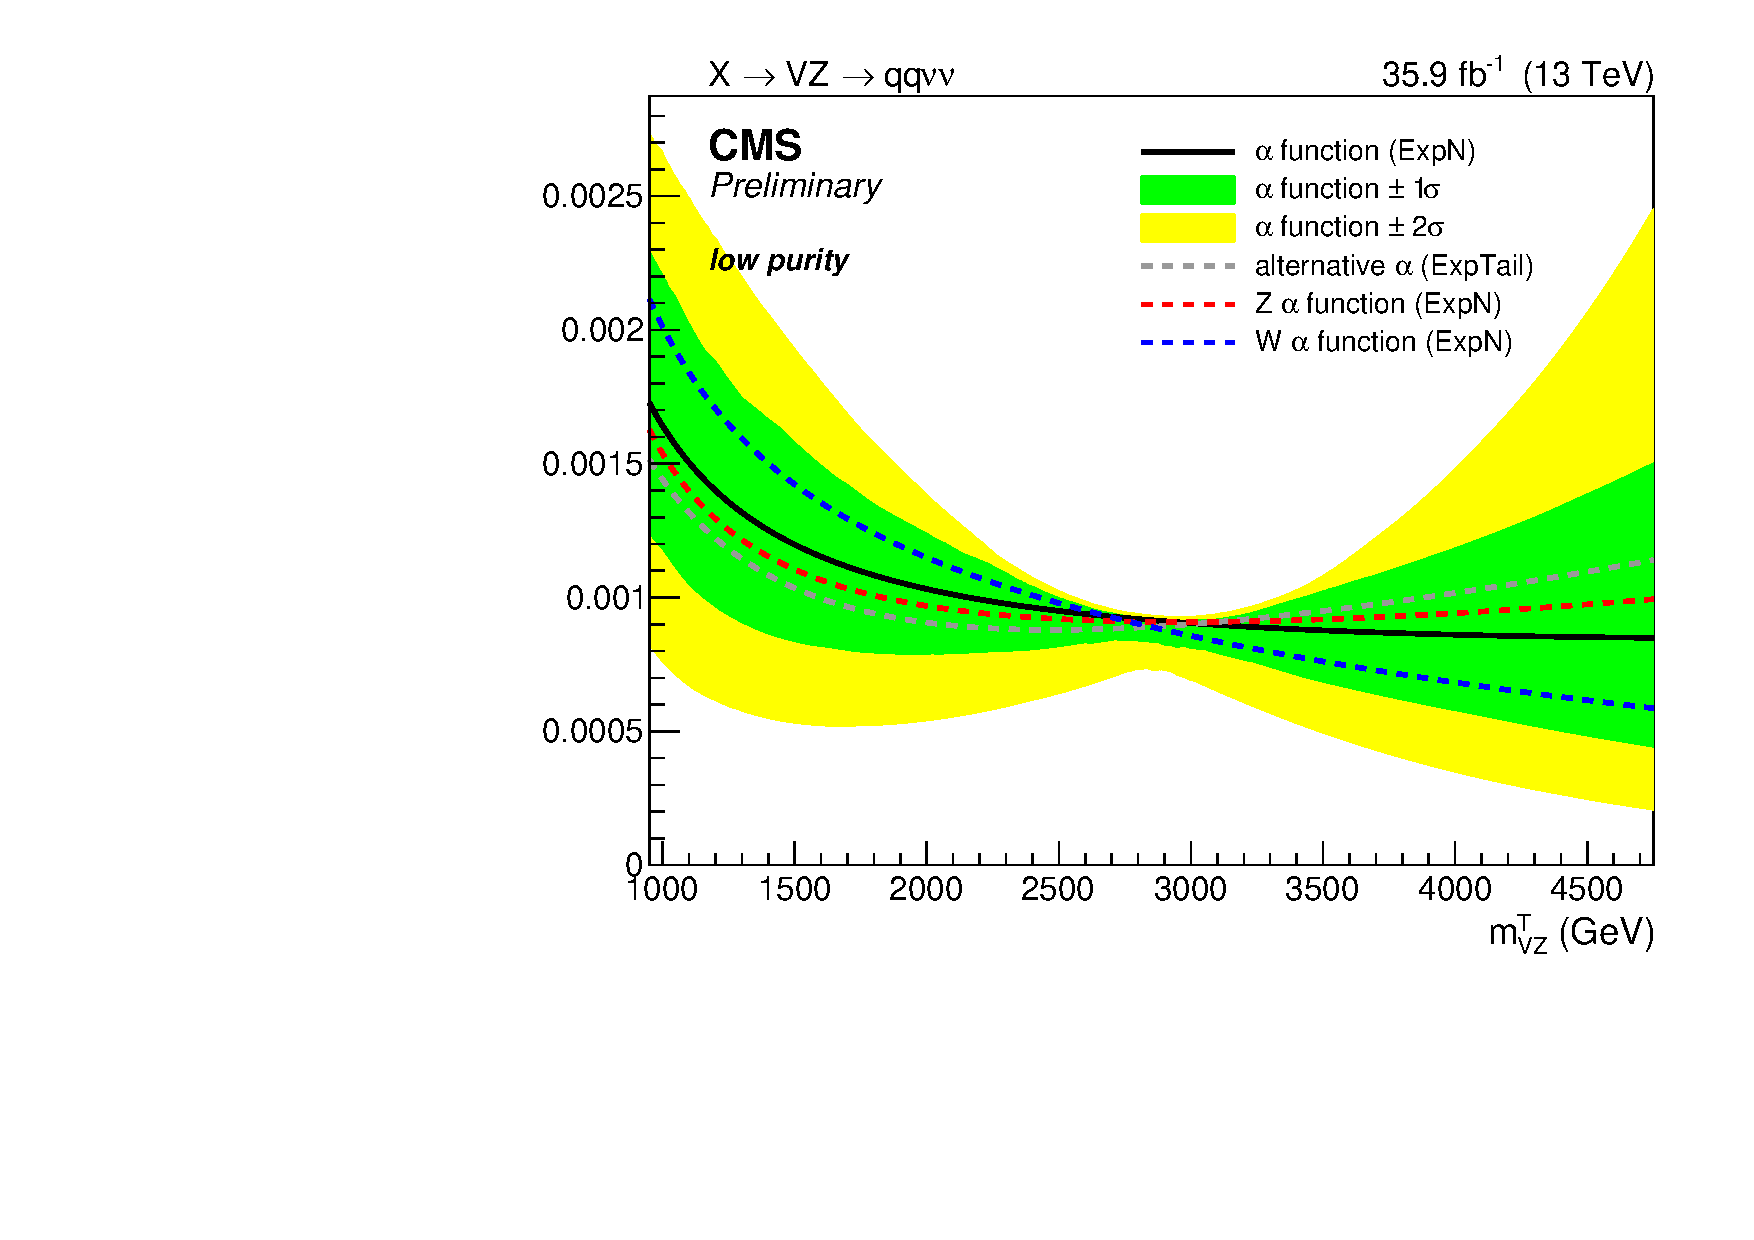
\includegraphics[width=.495\textwidth]{plotsAlpha_tesi/XVZnnlp/FourAlphaRatio.pdf}
    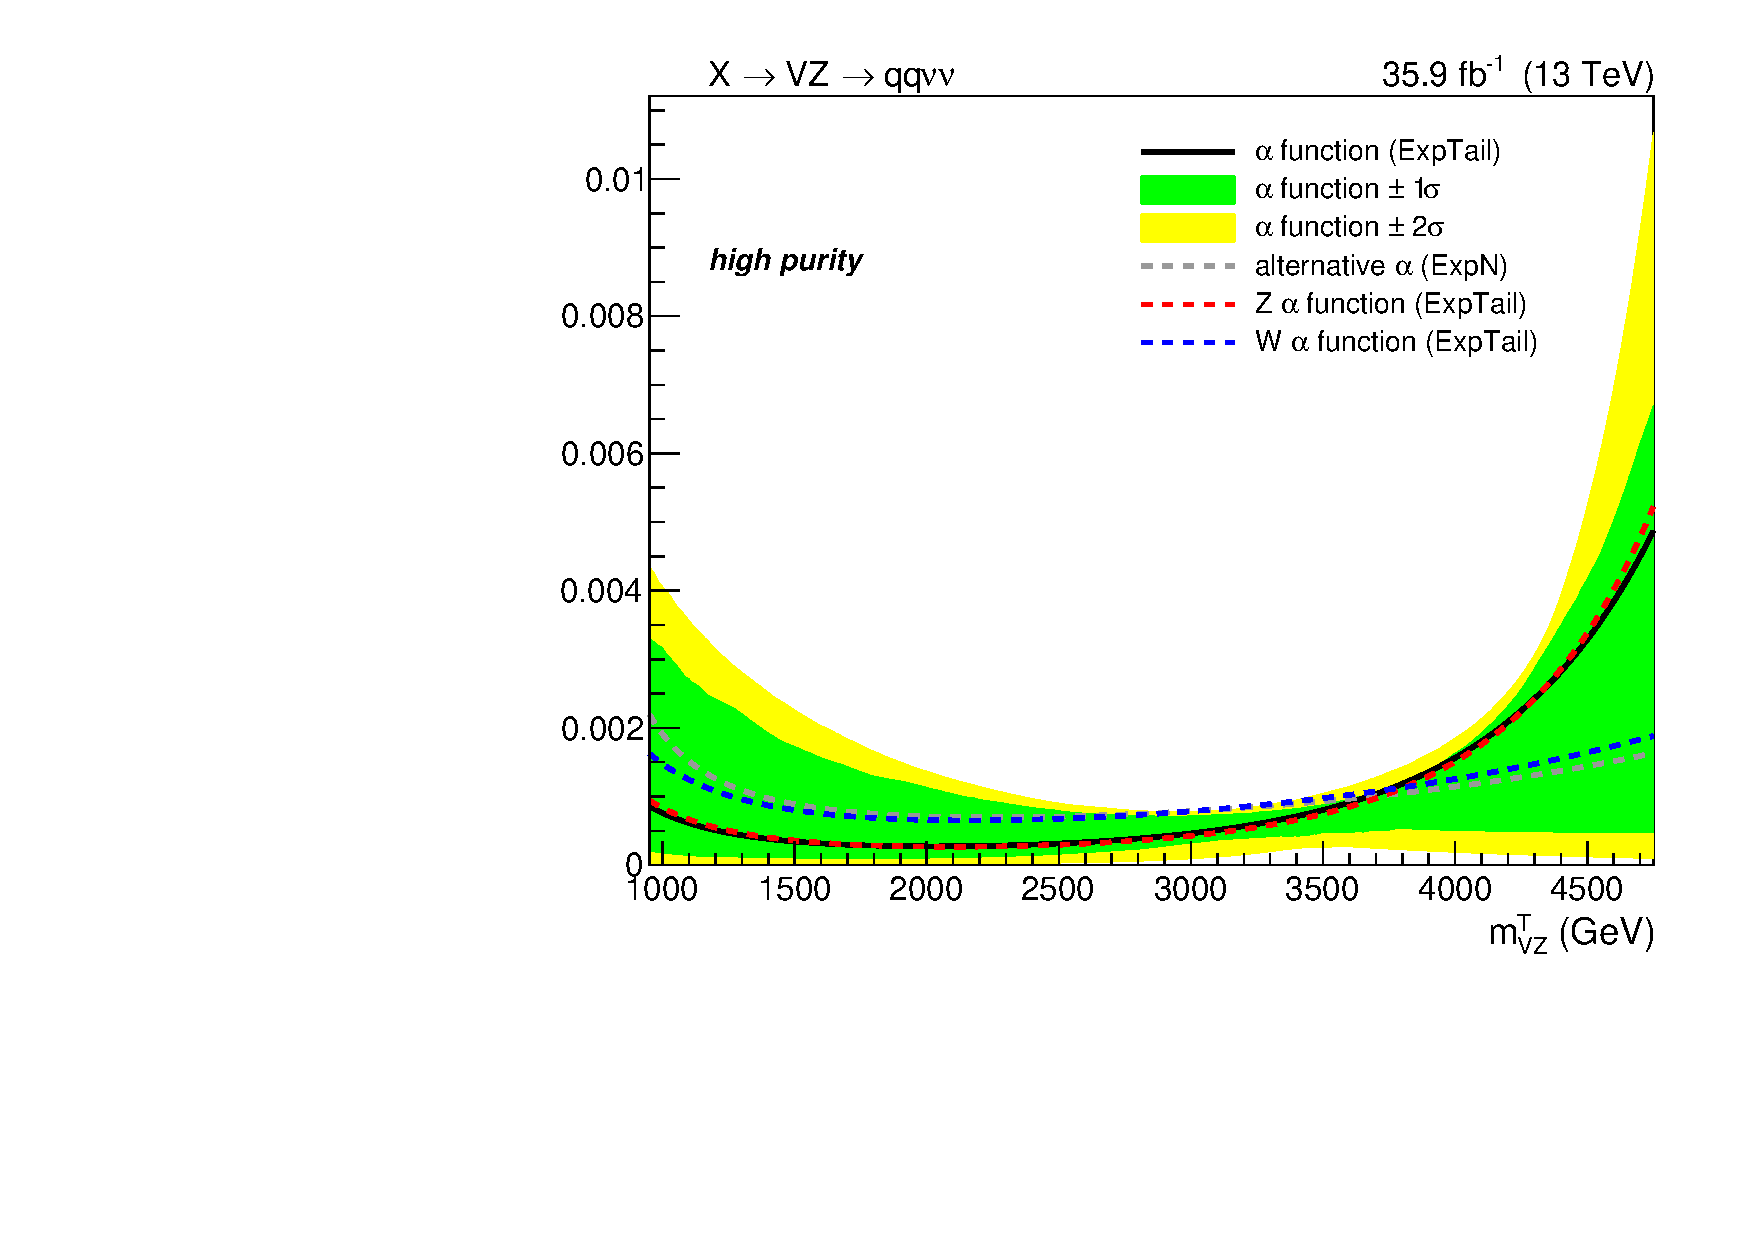
\includegraphics[width=.495\textwidth]{plotsAlpha_tesi/XVZnnhp/FourAlphaRatio.pdf}
  \caption{Validation of the $\alpha$ method: $\alpha$ functions calculated for \Z + jets background (red dotted line) and for \W + jets background (blue dotted line) separately, and $\alpha$ function for the \V + jets background merged together (black solid line). Left: low-purity category; right: high-purity category.}
  \label{fig:XVZnn_WZvalidation}
\end{figure}

The first required validation is performed in order to legitimate the choice of putting the \Z + jets and the \W + jets backgrounds together while performing the background estimation. The full procedure has been repeated, by keeping the two background contributions separated. Fit results performed on SB (top plots) and SR (bottom plots) of MC samples are displayed in fig.~\ref{fig:XVZnnlp_WZvalidation} (~\ref{fig:XVZnnhp_WZvalidation}) for low- (high-) purity category, for \Z + jets and \W jets background, separately, and for the combination of the two. In fig.~\ref{fig:XVZnn_WZvalidation}, the $\alpha$ functions calculated for \Z + jets background (red dotted line) and for \W + jets background (blue dotted line) are in agreement with the $\alpha$ function used in the analysis (black solid line), where the two backgrounds are merged together, both in low- (left plot) and high-purity category (right plot).


%\newpage
\vspace*{1\baselineskip}

\noindent As a robustness check of the $\alpha$-ratio method, a closure test is performed on data. Instead of predicting the background in the real SR form both the lower and the upper jet mass sidebands, the SB and SR are redefined for the purposes of this test. The low sideband is splitted in two sub-regions: $30-50~\GeV$ (LSB) and $50-65~\GeV$ (SR). The first is considered as the low sideband, while the latter is exploited as a pseudo-signal region. The high sideband is instead effectively used in the fit without any modifications with respect to the standard $\alpha$-ratio method. With this configuration, the prediction of the background in the SR region is estimated from the fit to the LSB region and the high-sidebands, and checked with data for both shape and normalization. This test has been performed before the unblinding of the signal region of the analysis.

\begin{table}[!htb]
  \begin{center}
    \begin{tabular}{cc|cc}
      region & category & Expected & Observed \\
      \hline
      \hline
      SB & low-purity & $1841.3 \pm 45.7$ & $1793$ \\
      SR & low-purity & $529.9 \pm 37.8$ & $521$ \\
      \hline
      SB & high-purity & $728.5 \pm 29.9$ & $725$ \\
      SR & high-purity & $39.3 \pm 5.2$ & $49$ \\
    \end{tabular}
  \end{center}
  \caption{Expected and observed background yield in the pseudo-SR jet mass region ($ 50 < m_j < 65\GeV$), predicted from the LSB one ($30 < m_j < 50\GeV$) and high-sideband ($m_j > 135~\GeV$).}\label{tab:alphaClosure}
\end{table}

\begin{figure}[!htb]
  \centering
    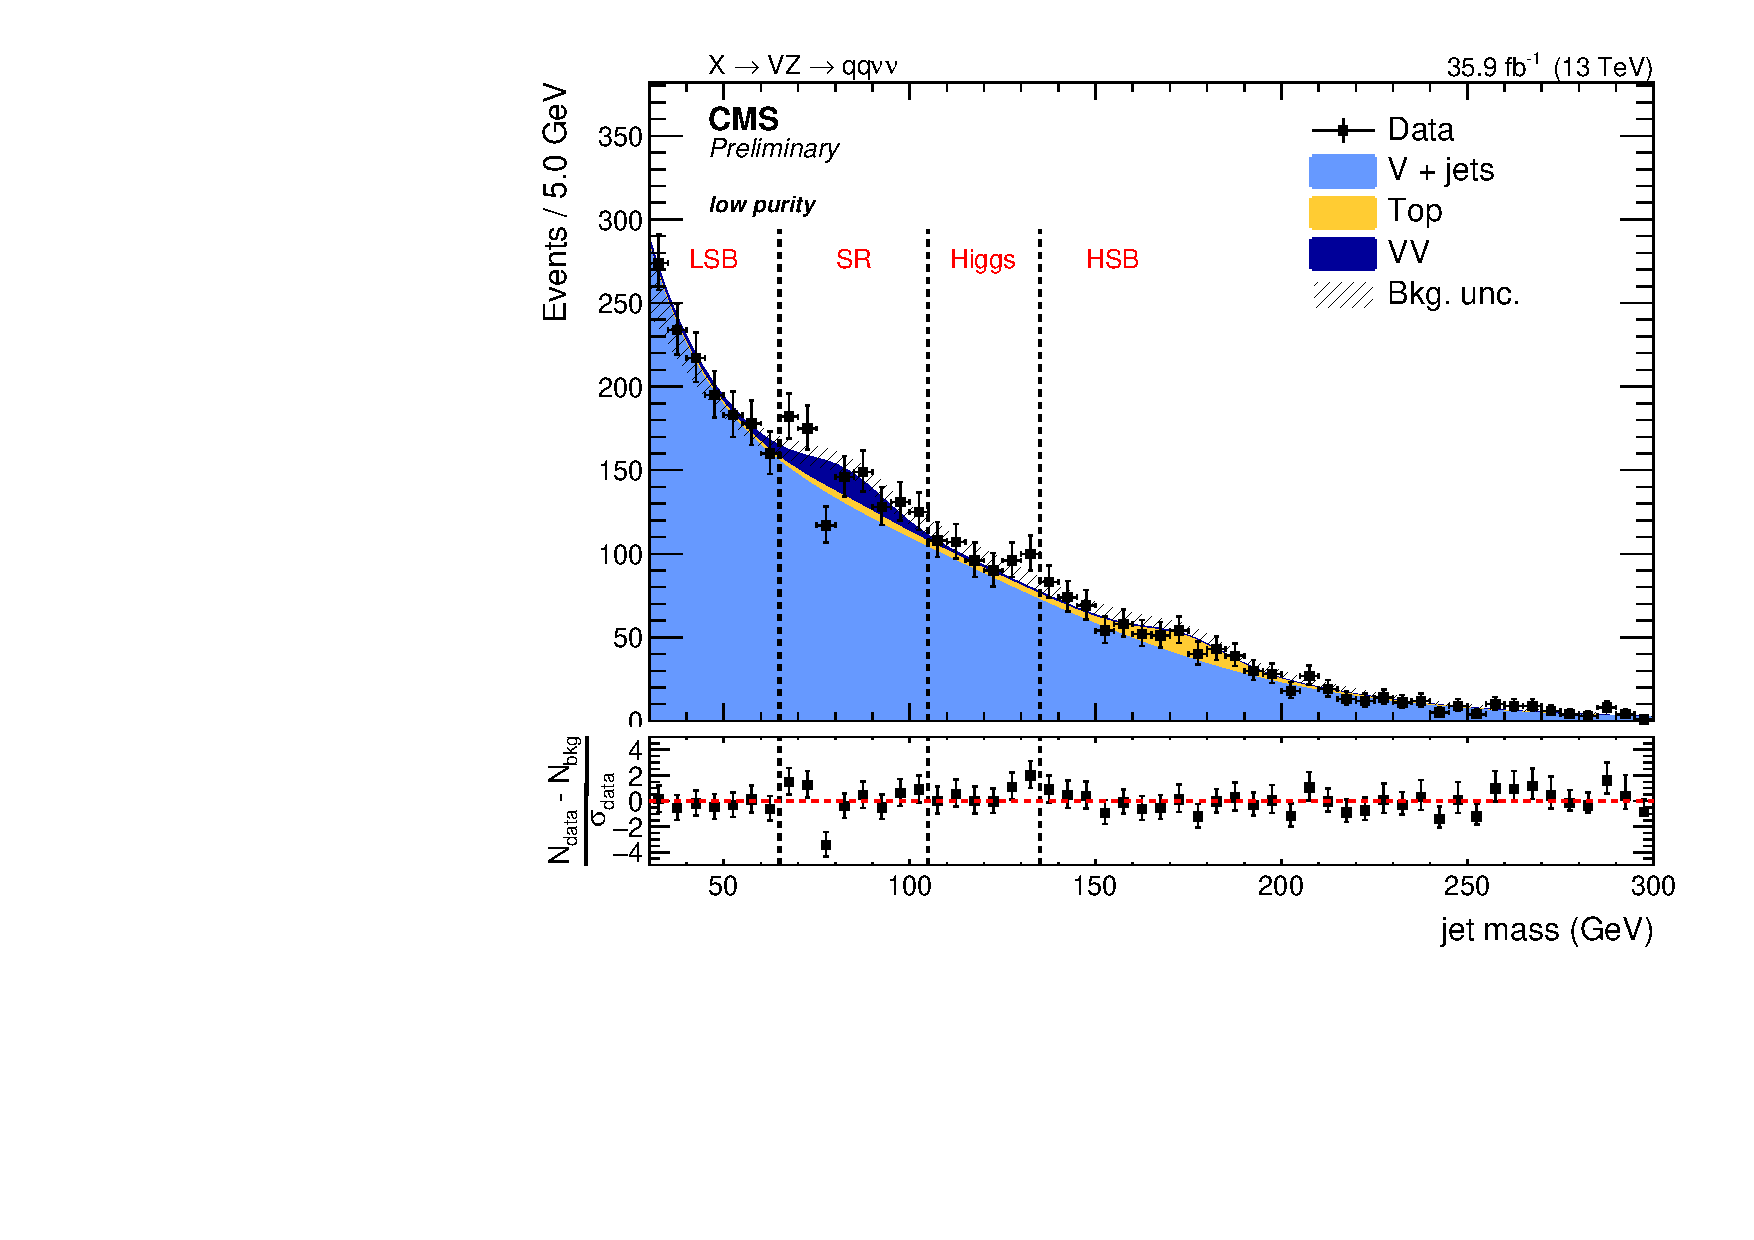
\includegraphics[width=.495\textwidth]{v9/plotsAlphaExt/XVZnnlp/XVZnnlp_JetMass.pdf}
    \includegraphics[width=.495\textwidth]{v9/plotsAlphaExt/XVZnnlp/BkgSR.pdf}%BkgSR.pdf}
    \\
    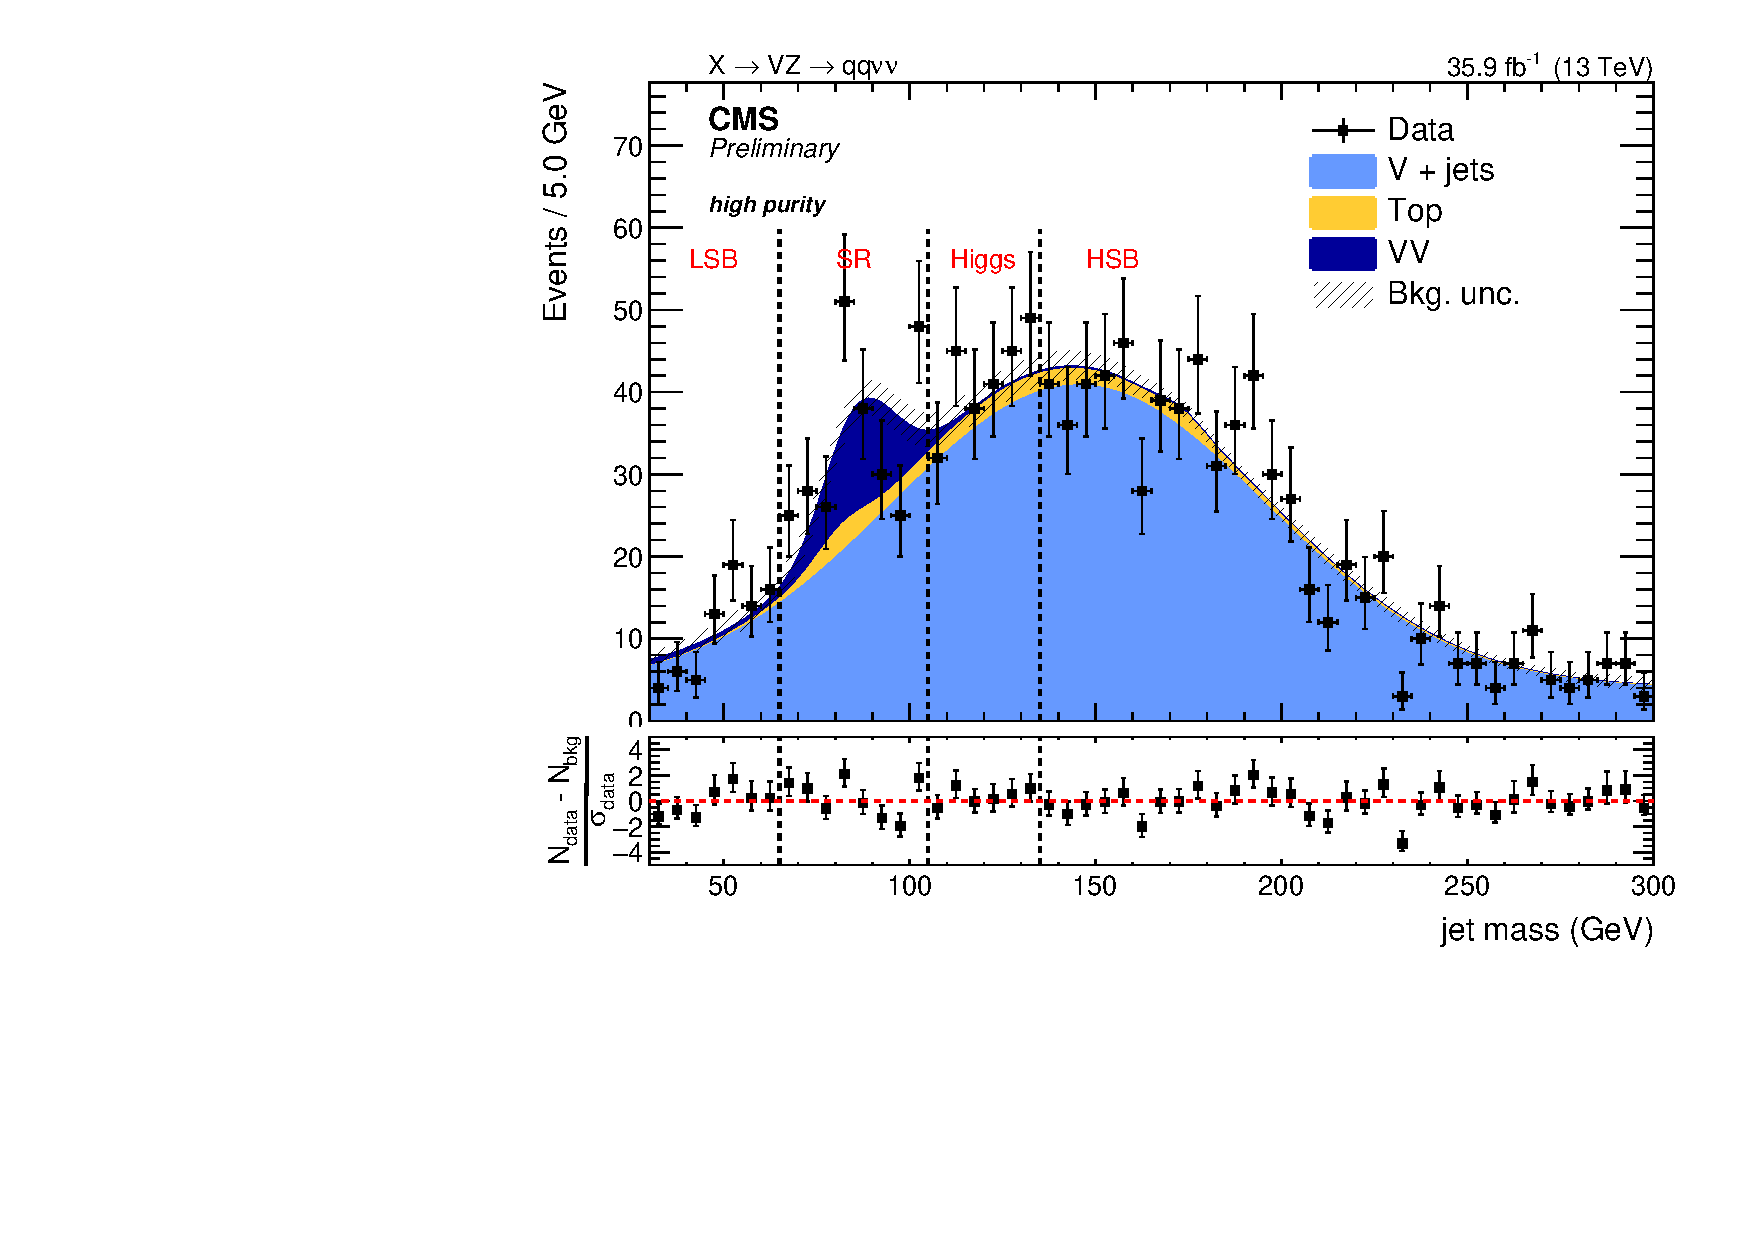
\includegraphics[width=.495\textwidth]{v9/plotsAlphaExt/XVZnnhp/XVZnnhp_JetMass.pdf}
    \includegraphics[width=.495\textwidth]{v9/plotsAlphaExt/XVZnnhp/BkgSR.pdf}%BkgSR.pdf}
  \caption{Top: fit to the $m_j$ spectrum in data in the sideband defined for the $\alpha$ method validation in the low-purity category: LSB ($30 < m_j < 50\GeV$) and high-sideband ($m_j > 135~\GeV$). Bottom: fit to the $m_j$ spectrum in data in the sideband defined for the $\alpha$ method validation in the high-purity category: LSB ($30 < m_j < 50\GeV$) and high-sideband ($m_j > 135~\GeV$). Both the signal region and the Higgs regions are kept blind, while the pseudo-signal is shown in the SR region ($50 < m_j < 65\GeV$).}
  \label{fig:alphaClosure}
\end{figure}

\noindent In fig.~\ref{fig:alphaClosure} and tab.~\ref{tab:alphaClosure}, the predicted shapes and normalizations are compared to the observed ones in data. 
A good overall agreement both in normalization and shape is obtained. There is a bit of tension in normalization for high-purity category, due to an upper fluctuation in data around 60 \GeV. This cross check confirms that the method to extract the \V+jets background is reliable and can be used to model the background in the search for potential excesses in the signal region defined in the analysis.

%\newpage
\vspace*{1\baselineskip}

\noindent The last check performed is a study of the impact of the choice of the function to describe the \V + jets background on the very last result of the analysis, namely the exclusion limit on the signal cross-section times branching ratio. The procedure of the limit extraction is discussed in detail in sec.~\ref{sec:results}. The main and alternative functions chosen to parametrize the dominant background depend on the purity category and are listed in tab.~\ref{tab:XMassFunctions}. In fig.~\ref{fig:validation_mainalt} (top), the fit results of the background shape prediction of the transverse mass are displayed. They are obtained by choosing the main function to describe the main background (red curve) and the alternative function (green curve); the two predictions are in agreement and very close to each other, for both low- (left) and high- (right) purity category. In fig.~\ref{fig:validation_mainalt} (center), the 95\% CL exclusion limits on cross-section times branching ratio are displayed for a spin-2 bulk graviton hypotesis, as a function of the mass of the resonance. The same figure of merit is shown in fig.~\ref{fig:validation_mainalt} (bottom), considering a spin-1 \Wp hypotesis. In the plots, the exclusion limits are calculated by chosing the main function to describe the \V + jets background (left plots: green curve for low-purity category alone and black curve for high-purity category alone, right plot: red curve for the combination of the categories) or the alternative function (left plots: orange curve for low-purity category alone and pink curve for high-purity category alone, right plot: blue curve for the combination of the categories). The impact of the choice of the function is negligible ($<<1 \%$).


\begin{figure}[!htb]
  \centering

    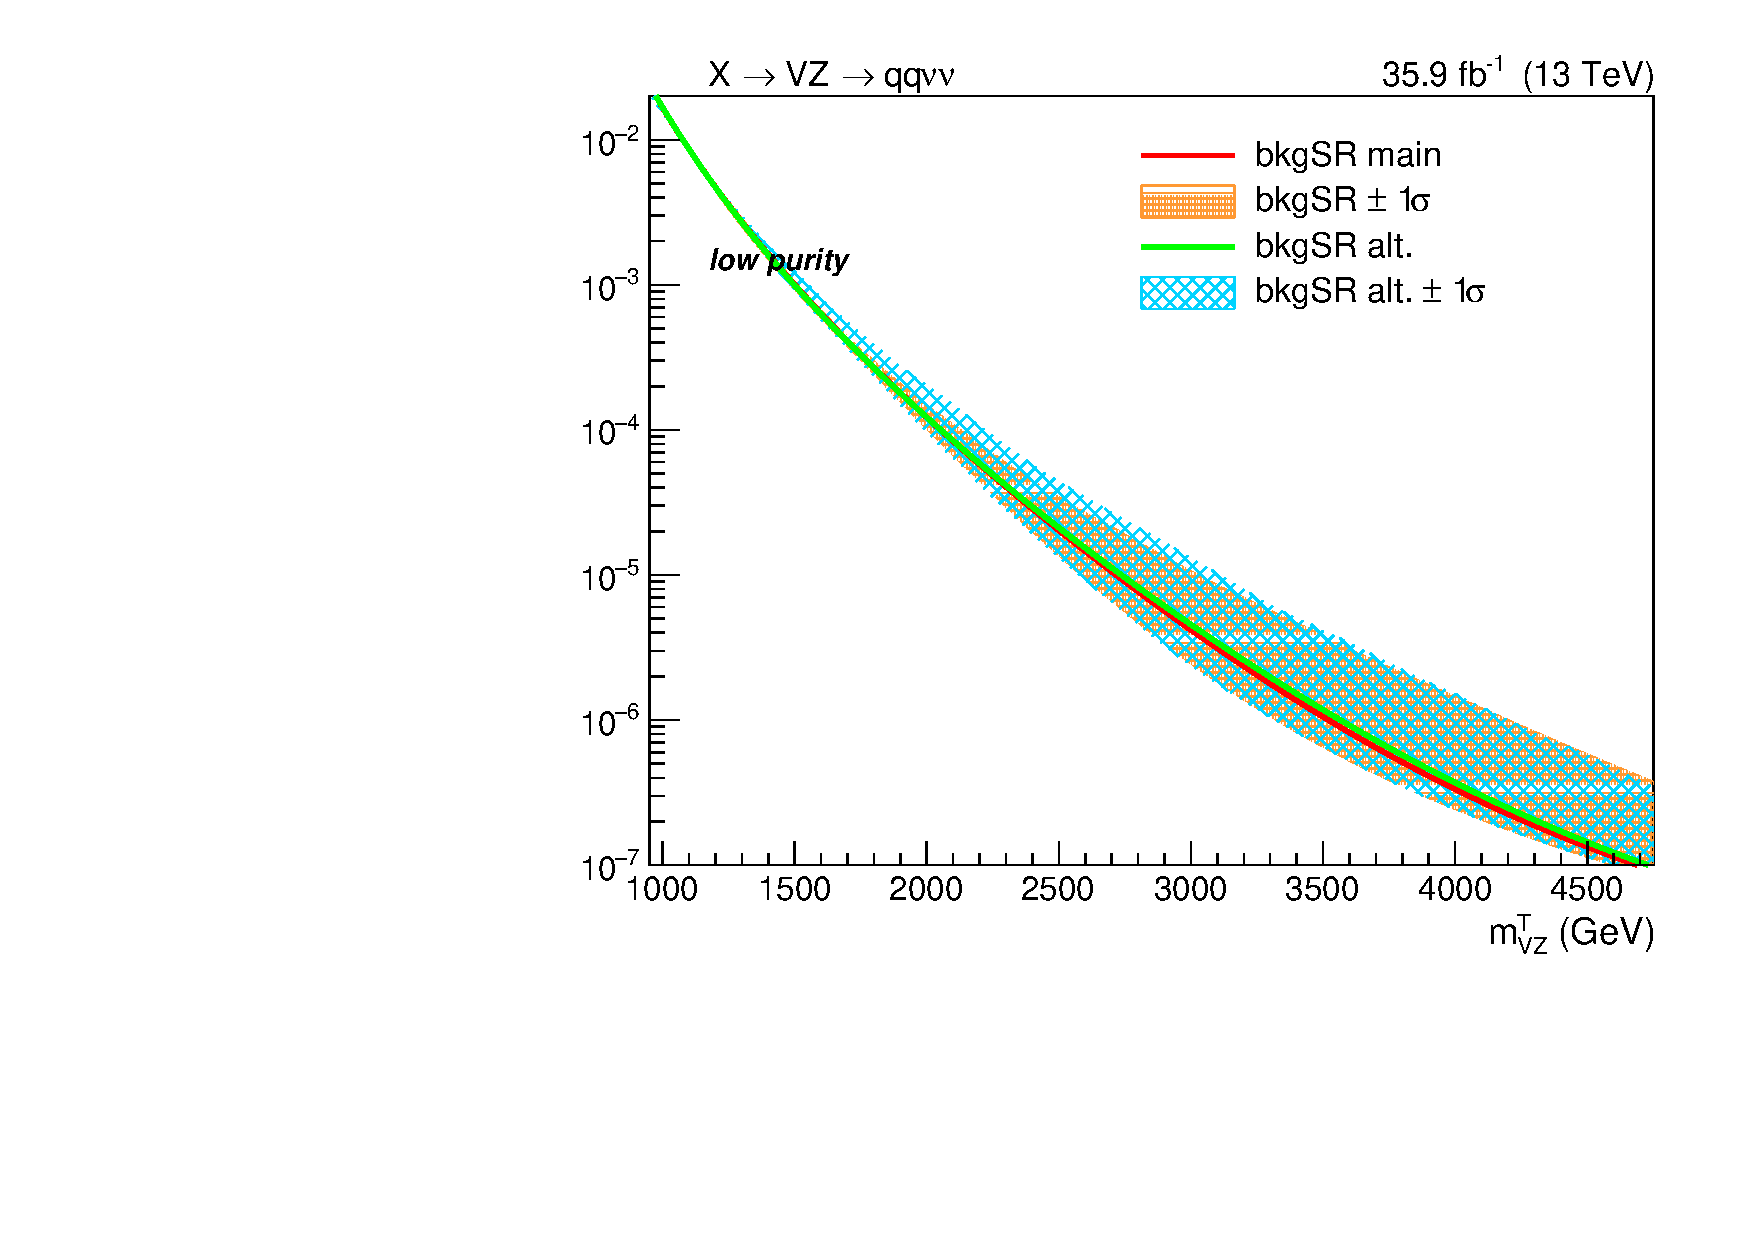
\includegraphics[width=.495\textwidth]{plotsAlpha_tesi/XVZnnlp/AlphaBiasSR.pdf}
    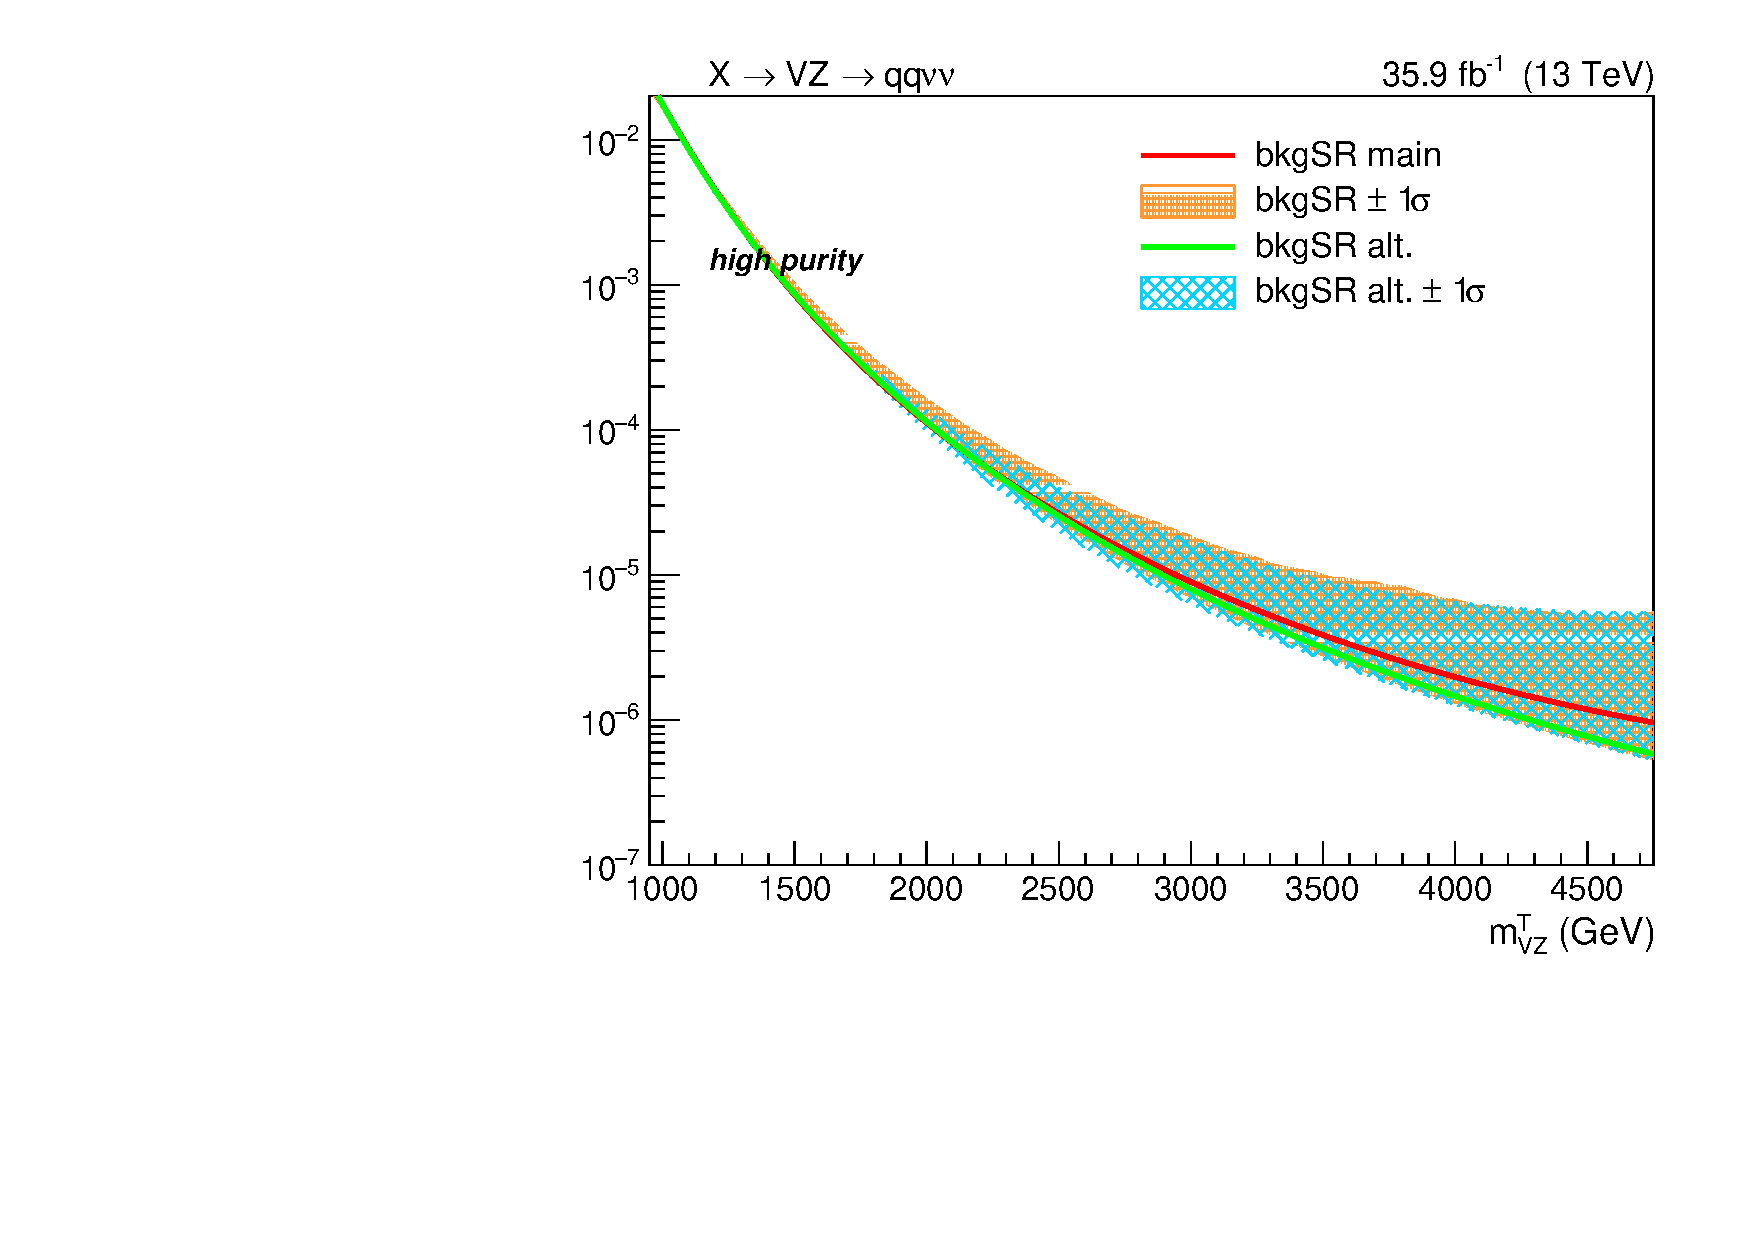
\includegraphics[width=.495\textwidth]{plotsAlpha_tesi/XVZnnhp/AlphaBiasSR.pdf}

    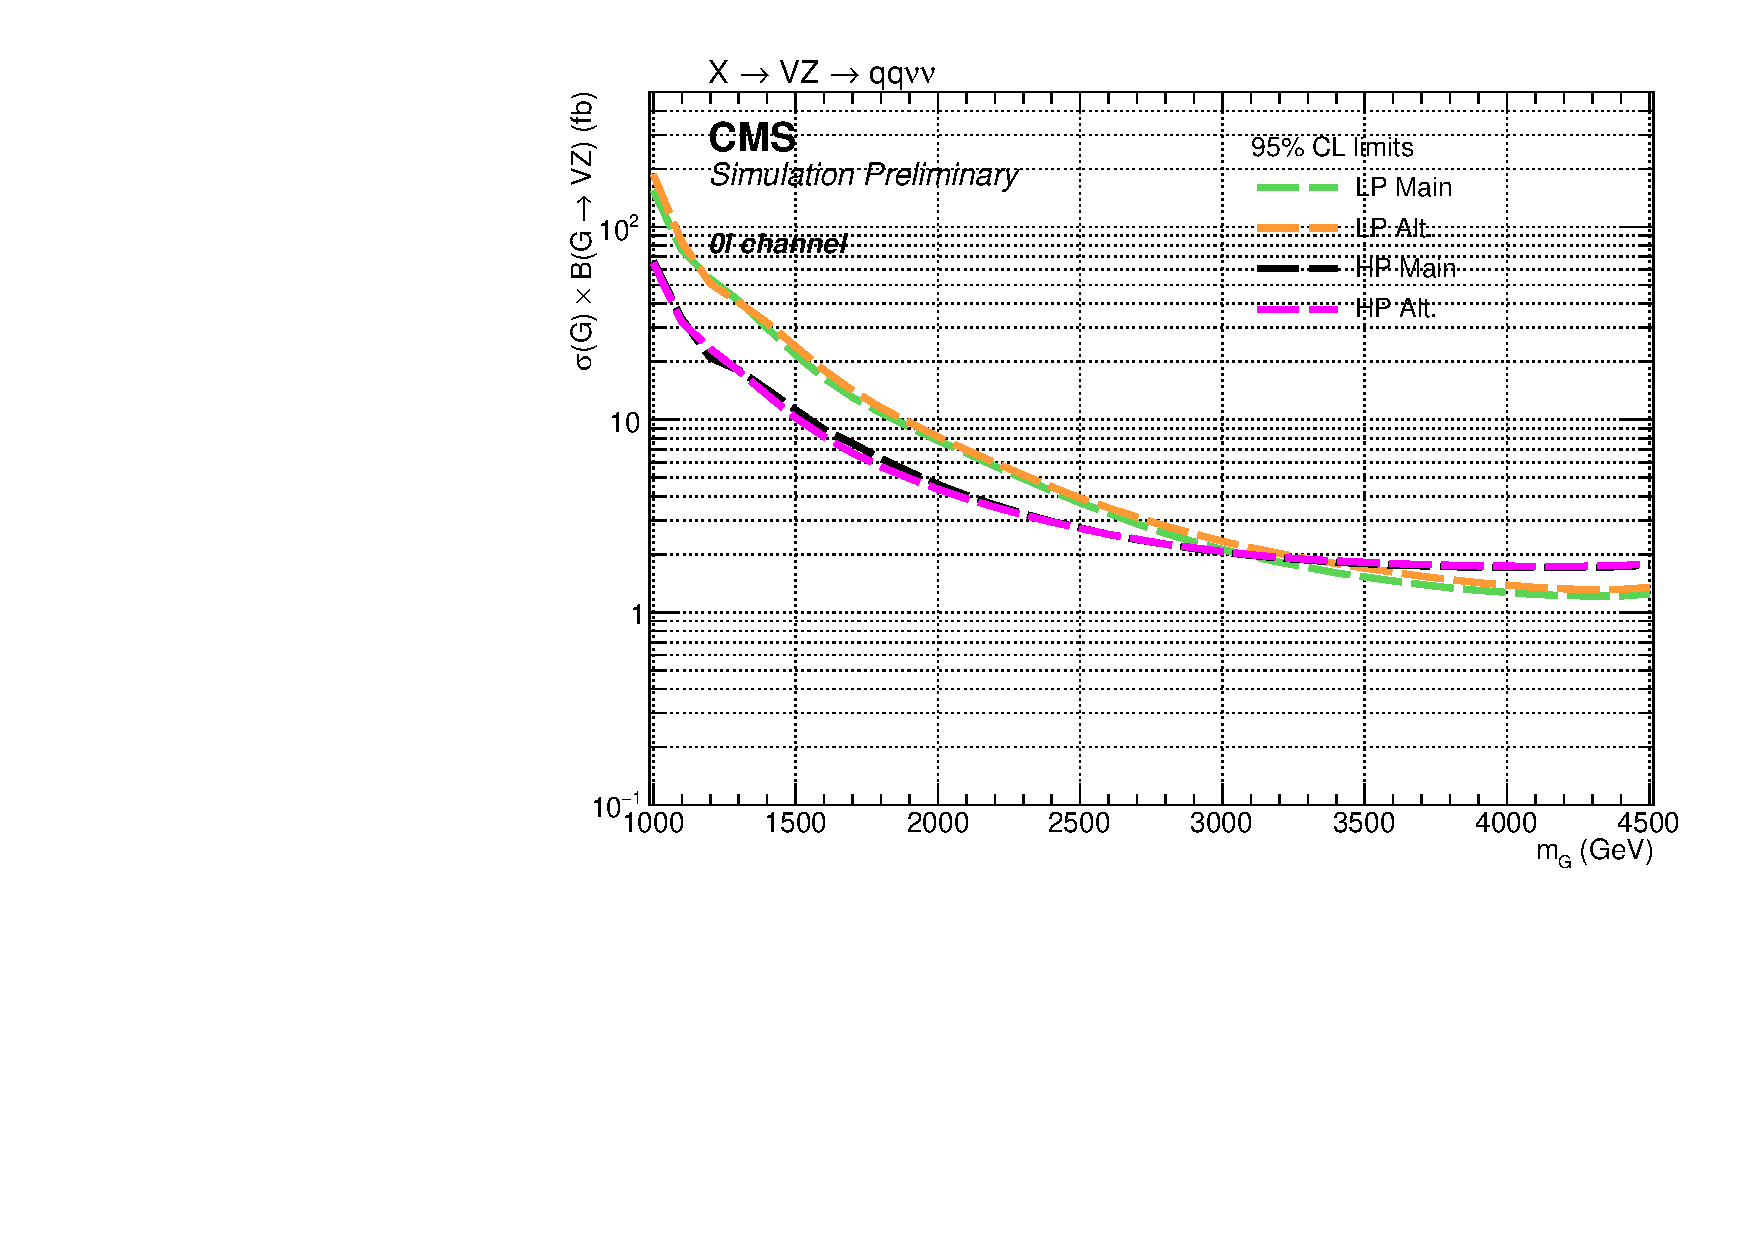
\includegraphics[width=.495\textwidth]{BackgroundFunctionValidation/Exclusion_XZZInv_main_vs_alt_LPHP_test.pdf}
    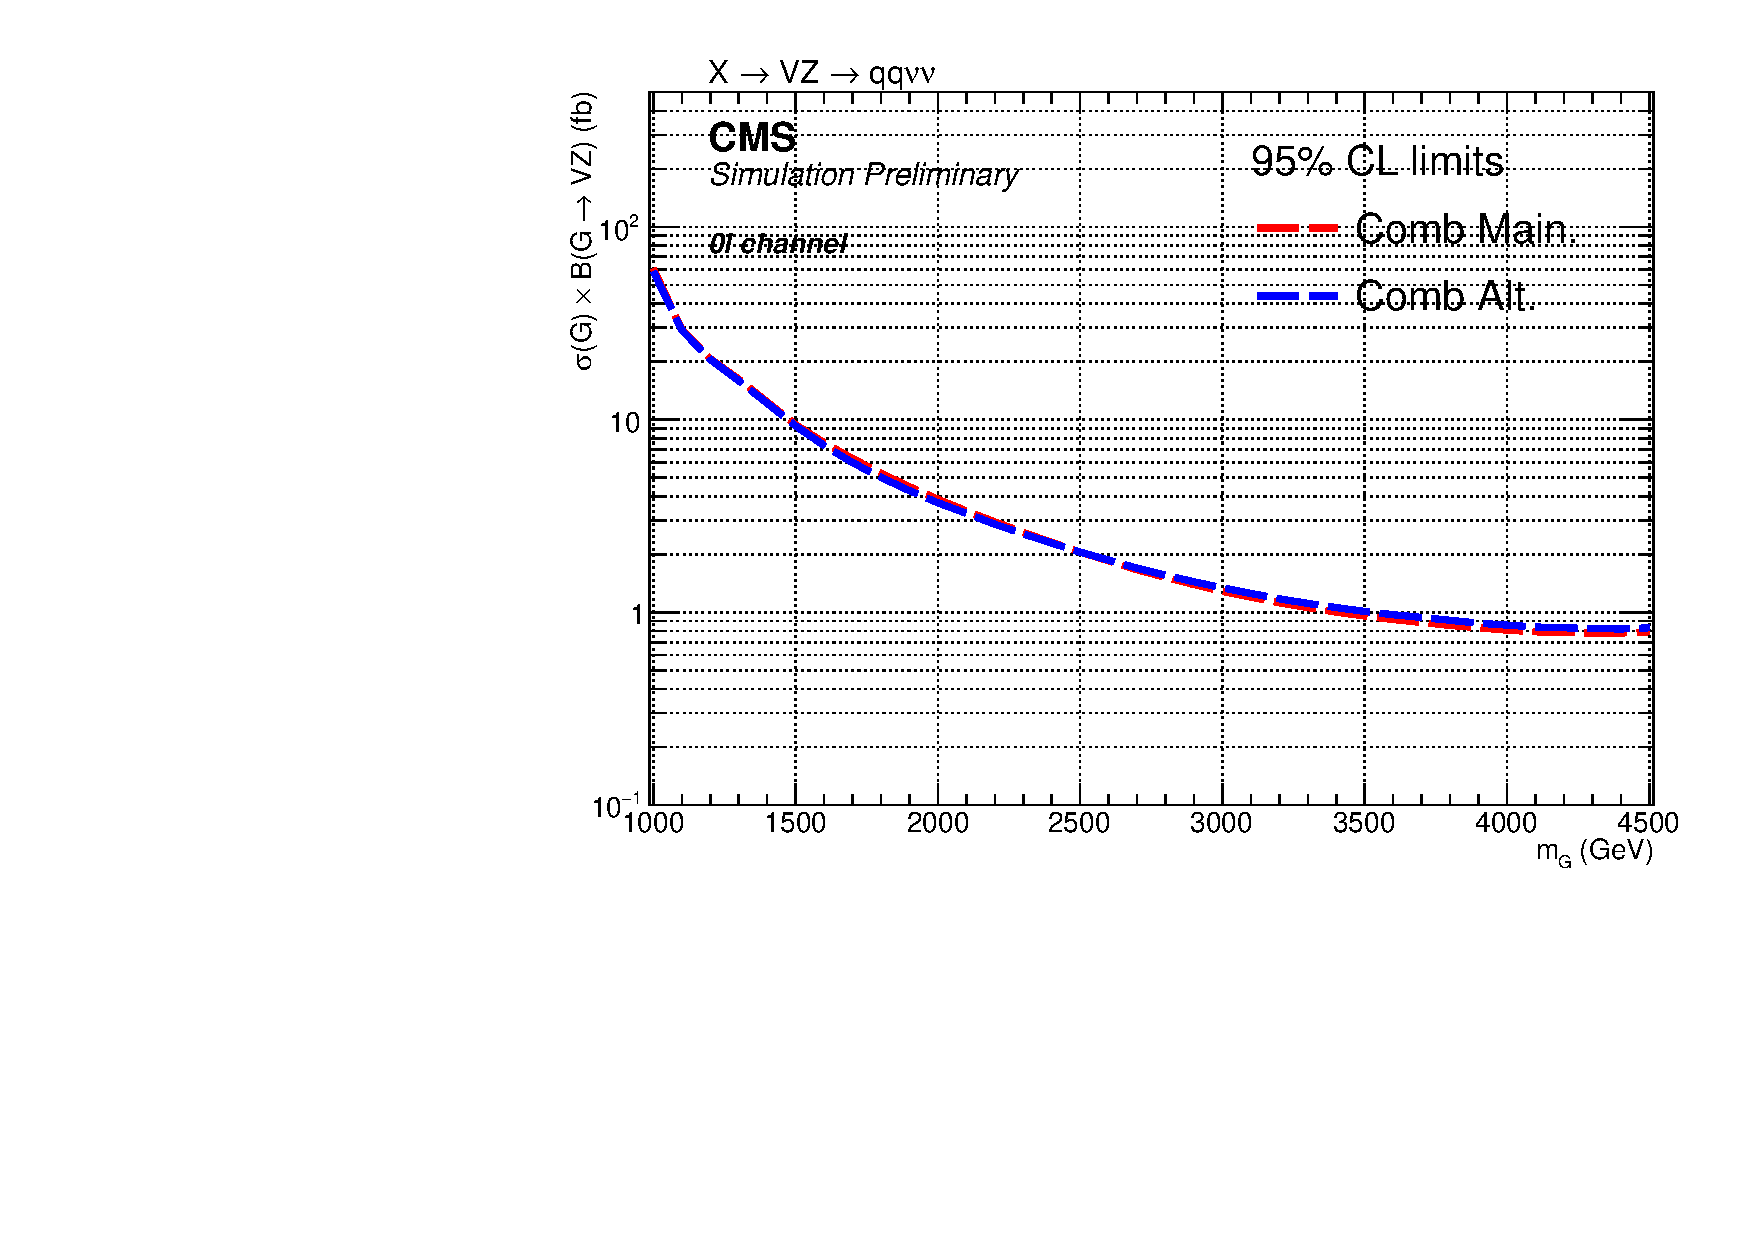
\includegraphics[width=.495\textwidth]{BackgroundFunctionValidation/Exclusion_XZZInv_main_vs_alt_comb_test.pdf}

    \includegraphics[width=.495\textwidth]{BackgroundFunctionValidation/Exclusion_XWZInv_main_vs_alt_LPHP_test.pdf}
    \includegraphics[width=.495\textwidth]{BackgroundFunctionValidation/Exclusion_XWZInv_main_vs_alt_comb_test.pdf}

  \caption{Validation of the $\alpha$ method: impact of the choice of the function to describe the dominant \V + jets background. Top: fit results of the background shape prediction in the SR obtained with the main function (red curve) and the alternative function (green curve), for low- (left) and high- (right) purity category. Center: exclusion limits on cross-section times branching ratio for a spin-2 bulk graviton hypotesis, as a function of the mass of the resonance, calculated by chosing the main function (left plots: green curve for low-purity category alone and black curve for high-purity category alone, right plot: red curve for the combination of the categories) or the alternative function (left plots: orange curve for low-purity category alone and pink curve for high-purity category alone, right plot: blue curve for the combination of the categories). Bottom: exclusion limits on cross-section times branching ratio for a spin-1 \Wp hypotesis.}
  \label{fig:validation_mainalt}
\end{figure}

\clearpage

%\newpage
\subsection{Signal modeling}

The simulated signal mass points are fitted in the SR with an empiric function in order to be able to perform an unbinned likelihood fit for the signal extraction. The function chosen to model the signal samples is a \emph{Crystal Ball} function~\cite{Oreglia:1980cs,Skwarnicki:1986xj}, which is composed by a gaussian-like peak plus a tail towards lower values. Both spin-2 (fig.~\ref{fig:XVZnnlp_Signal}-~\ref{fig:XVZnnhp_Signal}) and spin-1 (fig.~\ref{fig:XWZnnlp_Signal}-~\ref{fig:XWZnnhp_Signal}) signal samples are fitted.

%[FIXME: plots and fits in this section are obtained only for Bulk Graviton samples]

\begin{figure}[!htb]
  \centering
    \includegraphics[width=.33\textwidth]{v9/plotsAlphaPt035/XVZnnlp/XZZInv_M1000.pdf}
    \includegraphics[width=.33\textwidth]{v9/plotsAlphaPt035/XVZnnlp/XZZInv_M1200.pdf}
    \includegraphics[width=.33\textwidth]{v9/plotsAlphaPt035/XVZnnlp/XZZInv_M1400.pdf}
     \\
    \includegraphics[width=.33\textwidth]{v9/plotsAlphaPt035/XVZnnlp/XZZInv_M1600.pdf}
    \includegraphics[width=.33\textwidth]{v9/plotsAlphaPt035/XVZnnlp/XZZInv_M1800.pdf}
    \includegraphics[width=.33\textwidth]{v9/plotsAlphaPt035/XVZnnlp/XZZInv_M2000.pdf}
     \\
    \includegraphics[width=.33\textwidth]{v9/plotsAlphaPt035/XVZnnlp/XZZInv_M2500.pdf}
    \includegraphics[width=.33\textwidth]{v9/plotsAlphaPt035/XVZnnlp/XZZInv_M3000.pdf}
    \includegraphics[width=.33\textwidth]{v9/plotsAlphaPt035/XVZnnlp/XZZInv_M3500.pdf}
     \\
    \includegraphics[width=.33\textwidth]{v9/plotsAlphaPt035/XVZnnlp/XZZInv_M4000.pdf}
    \includegraphics[width=.33\textwidth]{v9/plotsAlphaPt035/XVZnnlp/XZZInv_M4500.pdf}
  \caption{Fit to the spin-2 (bulk graviton) signal samples in the low-purity category.}
  \label{fig:XVZnnlp_Signal}
\end{figure}


\begin{figure}[!htb]
  \centering
    \includegraphics[width=.33\textwidth]{v9/plotsAlphaPt035/XVZnnhp/XZZInv_M1000.pdf}
    \includegraphics[width=.33\textwidth]{v9/plotsAlphaPt035/XVZnnhp/XZZInv_M1200.pdf}
    \includegraphics[width=.33\textwidth]{v9/plotsAlphaPt035/XVZnnlp/XZZInv_M1400.pdf}
     \\
    \includegraphics[width=.33\textwidth]{v9/plotsAlphaPt035/XVZnnhp/XZZInv_M1600.pdf}
    \includegraphics[width=.33\textwidth]{v9/plotsAlphaPt035/XVZnnhp/XZZInv_M1800.pdf}
    \includegraphics[width=.33\textwidth]{v9/plotsAlphaPt035/XVZnnhp/XZZInv_M2000.pdf}
     \\
    \includegraphics[width=.33\textwidth]{v9/plotsAlphaPt035/XVZnnhp/XZZInv_M2500.pdf}
    \includegraphics[width=.33\textwidth]{v9/plotsAlphaPt035/XVZnnhp/XZZInv_M3000.pdf}
    \includegraphics[width=.33\textwidth]{v9/plotsAlphaPt035/XVZnnhp/XZZInv_M3500.pdf}
     \\
    \includegraphics[width=.33\textwidth]{v9/plotsAlphaPt035/XVZnnhp/XZZInv_M4000.pdf}
    \includegraphics[width=.33\textwidth]{v9/plotsAlphaPt035/XVZnnhp/XZZInv_M4500.pdf}
  \caption{Fit to the spin-2 (bulk graviton) signal samples in the high-purity category.}
  \label{fig:XVZnnhp_Signal}
\end{figure}

\begin{figure}[!htb]
  \centering
    \includegraphics[width=.33\textwidth]{v9/plotsAlphaPt035/XVZnnlp/XWZInv_M1000.pdf}
    \includegraphics[width=.33\textwidth]{v9/plotsAlphaPt035/XVZnnlp/XWZInv_M1200.pdf}
    \includegraphics[width=.33\textwidth]{v9/plotsAlphaPt035/XVZnnlp/XWZInv_M1400.pdf}
     \\
    \includegraphics[width=.33\textwidth]{v9/plotsAlphaPt035/XVZnnlp/XWZInv_M1600.pdf}
    \includegraphics[width=.33\textwidth]{v9/plotsAlphaPt035/XVZnnlp/XWZInv_M1800.pdf}
    \includegraphics[width=.33\textwidth]{v9/plotsAlphaPt035/XVZnnlp/XWZInv_M2000.pdf}
     \\
    \includegraphics[width=.33\textwidth]{v9/plotsAlphaPt035/XVZnnlp/XWZInv_M2500.pdf}
    \includegraphics[width=.33\textwidth]{v9/plotsAlphaPt035/XVZnnlp/XWZInv_M3000.pdf}
    \includegraphics[width=.33\textwidth]{v9/plotsAlphaPt035/XVZnnlp/XWZInv_M3500.pdf}
     \\
    \includegraphics[width=.33\textwidth]{v9/plotsAlphaPt035/XVZnnlp/XWZInv_M4000.pdf}
    \includegraphics[width=.33\textwidth]{v9/plotsAlphaPt035/XVZnnlp/XWZInv_M4500.pdf}
  \caption{Fit to the spin-1 (\Wp) signal samples in the low-purity category.}
  \label{fig:XWZnnlp_Signal}
\end{figure}


\begin{figure}[!htb]
  \centering
    \includegraphics[width=.33\textwidth]{v9/plotsAlphaPt035/XVZnnhp/XWZInv_M1000.pdf}
    \includegraphics[width=.33\textwidth]{v9/plotsAlphaPt035/XVZnnhp/XWZInv_M1200.pdf}
    \includegraphics[width=.33\textwidth]{v9/plotsAlphaPt035/XVZnnlp/XWZInv_M1400.pdf}
     \\
    \includegraphics[width=.33\textwidth]{v9/plotsAlphaPt035/XVZnnhp/XWZInv_M1600.pdf}
    \includegraphics[width=.33\textwidth]{v9/plotsAlphaPt035/XVZnnhp/XWZInv_M1800.pdf}
    \includegraphics[width=.33\textwidth]{v9/plotsAlphaPt035/XVZnnhp/XWZInv_M2000.pdf}
     \\
    \includegraphics[width=.33\textwidth]{v9/plotsAlphaPt035/XVZnnhp/XWZInv_M2500.pdf}
    \includegraphics[width=.33\textwidth]{v9/plotsAlphaPt035/XVZnnhp/XWZInv_M3000.pdf}
    \includegraphics[width=.33\textwidth]{v9/plotsAlphaPt035/XVZnnhp/XWZInv_M3500.pdf}
     \\
    \includegraphics[width=.33\textwidth]{v9/plotsAlphaPt035/XVZnnhp/XWZInv_M4000.pdf}
    \includegraphics[width=.33\textwidth]{v9/plotsAlphaPt035/XVZnnhp/XWZInv_M4500.pdf}
  \caption{Fit to the spin-1 (\Wp) signal samples in the high-purity category.}
  \label{fig:XWZnnhp_Signal}
\end{figure}


%\clearpage

\subsubsection{Signal parametrization}

The signal is parametrized by interpolating the fitted parameters separately for each channel in order to have a continous variation of the signal shape for every possible \mtVZ value within the range. A linear fit is performed on the mean and the width of the Gaussian core of the Crystal Ball functions. The interpolations are shown in fig.~\ref{fig:XZZ_SignalShapeLP}-~\ref{fig:XZZ_SignalShapeHP} for the spin-2 signal model, and in fig.~\ref{fig:XWZ_SignalShapeLP}-~\ref{fig:XWZ_SignalShapeHP} for the spin-1 signal model. Shape systematic uncertainties, as described in sec.~\ref{sec:uncertainties}, are taken into account while describing the mean and sigma of the gaussian core, and they are related to the effects of the jet mass scale and resolution. Other shape parameters describing the tails of the Crystal Ball are fitted as 3rd degree polynomial.

%[FIXME: since some Crystal Ball fits are partially failing, some parameters have awkward uncertainties, so the polynomial function is off, especially for the exponential slope parameter (bottom right). In this case, the SPLINE approach is chosen.]

\begin{figure}[!htb]
  \centering
    \includegraphics[width=.95\textwidth]{v9/plotsAlphaPt035/XVZnnlp/XZZInv_SignalShape.pdf}
  \caption{Interpolation of the fitted parameters as a function of the generated mass \mtVZ, for a spin-2 (bulk graviton) signal hypothesis, low-purity category.}
  \label{fig:XZZ_SignalShapeLP}
\end{figure}

\begin{figure}[!htb]
  \centering
    \includegraphics[width=.95\textwidth]{v9/plotsAlphaPt035/XVZnnhp/XZZInv_SignalShape.pdf}

  \caption{Interpolation of the fitted parameters as a function of the generated mass \mtVZ, for a spin-2 (bulk graviton) signal hypothesis, high-purity category.}
  \label{fig:XZZ_SignalShapeHP}
\end{figure}

\begin{figure}[!htb]
  \centering
    \includegraphics[width=.95\textwidth]{v9/plotsAlphaPt035/XVZnnlp/XWZInv_SignalShape.pdf}
  \caption{Interpolation of the fitted parameters as a function of the generated mass \mtVZ, for a spin-1 (\Wp) signal hypothesis, low-purity category.}
  \label{fig:XWZ_SignalShapeLP}
\end{figure}

\begin{figure}[!htb]
  \centering
    \includegraphics[width=.95\textwidth]{v9/plotsAlphaPt035/XVZnnhp/XWZInv_SignalShape.pdf}

  \caption{Interpolation of the fitted parameters as a function of the generated mass \mtVZ, for a spin-1 (\Wp) signal hypothesis, high-purity category.}
  \label{fig:XWZ_SignalShapeHP}
\end{figure}


\noindent The normalization of the signal samples is extrapolated from the fitted integral of the Crystal Ball functions. The points are then connected with a line, in order to have an acceptable description of the normalization as a function of \mtVZ. The interpolations are shown in fig.~\ref{fig:XZZ_SignalNorm} for the spin-2 signal model, and in fig.~\ref{fig:XWZ_SignalNorm} for the spin-1 signal model.% and Fig.~\ref{fig:XWZ_SignalNorm}.

\begin{figure}[!htb]
  \centering
    \includegraphics[width=.495\textwidth]{v9/plotsAlphaPt035/XVZnnlp/XZZInv_SignalNorm.pdf}
    \includegraphics[width=.495\textwidth]{v9/plotsAlphaPt035/XVZnnhp/XZZInv_SignalNorm.pdf}
  \caption{Interpolation of the signal normalization as a function of the generated mass \mtVZ, for a spin-2 (Bulk Graviton) signal hypothesis. From left to right: low-purity, high-purity.}
  \label{fig:XZZ_SignalNorm}
\end{figure}

\begin{figure}[!htb]
  \centering
    \includegraphics[width=.495\textwidth]{v9/plotsAlphaPt035/XVZnnlp/XWZInv_SignalNorm.pdf}
    \includegraphics[width=.495\textwidth]{v9/plotsAlphaPt035/XVZnnhp/XWZInv_SignalNorm.pdf}
  \caption{Interpolation of the signal normalization as a function of the generated mass \mtVZ, for a spin-1 ($W^{'}$) signal hypothesis. From left to right: low-purity, high-purity.}
  \label{fig:XWZ_SignalNorm}
\end{figure}

\begin{figure}[!htb]
  \centering
    \includegraphics[width=.495\textwidth]{v9/plotsAlphaPt035/XVZnnlp/XZZInv_Signal.pdf}
    \includegraphics[width=.495\textwidth]{v9/plotsAlphaPt035/XVZnnhp/XZZInv_Signal.pdf}
  \caption{Interpolation of the signal as a function of the generated mass \mtVZ, for a spin-2 (Bulk Graviton) signal hypothesis with an arbitrary cross section of 1 \pb in the low- (left) and high-purity category (right).}
  \label{fig:XZZInv_Signal}
\end{figure}

\begin{figure}[!htb]
  \centering
    \includegraphics[width=.495\textwidth]{v9/plotsAlphaPt035/XVZnnlp/XWZInv_Signal.pdf}
    \includegraphics[width=.495\textwidth]{v9/plotsAlphaPt035/XVZnnhp/XWZInv_Signal.pdf}
  \caption{Interpolation of the signal as a function of the generated mass \mtVZ, for a spin-1 ($W^{'}$) signal hypothesis with an arbitrary cross section of 1 \pb in the low- (left) and high-purity category (right).}
  \label{fig:XWZInv_Signal}
\end{figure}

\clearpage

